\documentclass[11pt, a4paper]{report}
%\documentclass[11pt,a4paper,oneside]{report}

%Packages
\usepackage[hungarian]{babel}
\usepackage[utf8]{inputenc}
\usepackage{graphicx}
%
\usepackage{hyperref}
\usepackage{wrapfig}
\usepackage{subfigure }
\usepackage[margin=80pt]{geometry}
\usepackage{geometry}
\usepackage{amsmath}
\usepackage{tabularx}
\usepackage{tabulary}
%\usepackage{url}
\usepackage{multicol}
\usepackage{multirow}
\usepackage{setspace}
\usepackage[table,xcdraw]{xcolor}
%\usepackage[acronym]{glossaries}
\usepackage{longtable}
\usepackage{titlesec}



\usepackage[procnames]{listings}
\usepackage{color}


\definecolor{keywords}{RGB}{255,0,90}
\definecolor{green}{RGB}{0,0,113}
\definecolor{red}{RGB}{160,0,0}
\definecolor{comments}{RGB}{0,150,0}
 
\lstset{
    frame=single,
    breaklines=true,
    postbreak=\raisebox{0ex}[0ex][0ex]{\ensuremath{\color{red}\hookrightarrow\space}}
}

\lstset{language=Python, 
        basicstyle=\ttfamily\small, 
        keywordstyle=\color{keywords},
        commentstyle=\color{comments},
        stringstyle=\color{red},
        showstringspaces=false,
        identifierstyle=\color{green},
        procnamekeys={def,class}}

\pagestyle{plain}
\setlength{\parindent}{12pt} % magyar nyelvû dokumentumokban jellemzõ
\setlength{\parskip}{0pt}    % magyar nyelvû dokumentumokban jellemzõ
\frenchspacing
\setlength{\columnsep}{1cm}
\linespread{1.5}

\includeonly{
	cimlap,
	nyilatkozat,
	eloszo,
    internet,
    mereselmelet,
    felderites,
    meres,
    fejlesztes,
    eredmenyek,
    feldolgozas,
    egyuttmukodesek,
	zaras,
	fuggelek,
}
%%%%%%%%%%%%%%%%%%%%%%%%%%%%%%%%%%%%%%%%%


\begin{document}

%------------------------------------------------
% Eleje (4 oldal): tartalomjegyzék, abstract, bevezető, borító, stb...

%--------------------------------------------------------------------------------------
%	The title page
%--------------------------------------------------------------------------------------
\begin{titlepage}
\begin{center}

\includegraphics[width=60mm,keepaspectratio]{figures/BMElogo.png}\\
\vspace{0.3cm}
\textbf{Budapesti Műszaki és Gazdaságtudományi Egyetem}\\
\textmd{Villamosmérnöki és Informatikai Kar}\\
\textmd{Távközlési és Médiainformatikai Tanszék}\\[2.5cm]

\vspace{0.5cm}
\textsc{\LARGE Diplomaterv 1}\\[0.1cm]
\textsc{2015/16. tanév, 2. félév}\\[1.5cm]
\vspace{0.4cm}
{\huge \bfseries Automatizált internetes mérések}\\[5cm]

\begin{tabular}{cc}
 \makebox[7cm]{\emph{Készítette}} & \makebox[7cm]{\emph{Konzulens}} \\
 \makebox[7cm]{Horváth Rudolf} & \makebox[7cm]{Dr Heszberger Zalán}
\\
 \makebox[7cm]{rudolf.official@gmail.com} & \makebox[7cm]{heszberger@tmit.bme.hu}
 \\
 \makebox[7cm]{TS48JK} & \makebox[7cm]{}
\end{tabular}

\vfill
{\large \today}
\end{center}
\end{titlepage}




\tableofcontents

%--------------------------------------------------------------------------------------
% Nyilatkozat
%--------------------------------------------------------------------------------------
\begin{center}
\large
\textbf{HALLGATÓI NYILATKOZAT}\\
\end{center}

Alulírott \emph{Horváth Rudolf}, szigorló hallgató kijelentem, hogy ezt a diplomatervet meg nem engedett segítség nélkül, saját magam készítettem, csak a megadott forrásokat (szakirodalom, eszközök stb.) használtam fel. Minden olyan részt, melyet szó szerint, vagy azonos értelemben, de átfogalmazva más forrásból átvettem, egyértelmûen, a forrás megadásával megjelöltem.

Hozzájárulok, hogy a jelen munkám alapadatait (szerzõ(k), cím, angol és magyar nyelvû tartalmi kivonat, készítés éve, konzulens(ek) neve) a BME VIK nyilvánosan hozzáférhetõ elektronikus formában, a munka teljes szövegét pedig az egyetem belsõ hálózatán keresztül (vagy autentikált felhasználók számára) közzétegye. Kijelentem, hogy a benyújtott munka és annak elektronikus verziója megegyezik. Dékáni engedéllyel titkosított diplomatervek esetén a dolgozat szövege csak 3 év eltelte után válik hozzáférhetõvé.

\begin{flushleft}
\vspace*{1cm}
Budapest, \today
\end{flushleft}

\begin{flushright}
 \vspace*{1cm}
 \makebox[7cm]{\rule{6cm}{.4pt}}\\
 \makebox[7cm]{\emph{Horváth Rudolf}}\\
 \makebox[7cm]{hallgató}
\end{flushright}
\thispagestyle{empty}

\vfill
\clearpage
\thispagestyle{empty} % an empty page



\chapter*{Kivonat}\addcontentsline{toc}{chapter}{Kivonat}
%1 oldalas összefoglalása a munkának \textbf{Magyarul}.

Az internet olyan kulcsfontosságú infrastruktúra napjainkban, amelynek fontos ismerni az állapotát és viselkedését. Ezen Diplomamunka az internetes útvonalak vizsgálatával foglalkozik.
Egy automatizált Internetes mérési rendszer készült ennek érdekében, amely a PlanetLab szervezet gépeit felhasználva méréseket végez és monitorozza az internet általuk látható részeit. A mérési rendszer több mérési funkcióval rendelkezik. A begyűjtött adatok több feldolgozási folyamaton mennek keresztül, melyek egyik kimenete például útvonal változásokat elemez. A megbízható adatszolgáltatás érdekében a mérési rendszer folyamatos és hibatűrő működésre lett tervezve, felügyeleti funkciókkal kiegészítve. A felhasznált technológiák és az elkészült szoftverkomponensek nyílt forráskódú licensszel rendelkeznek, így mások is használhatják azokat, illetve bővíthetik saját fejlesztéseikkel.
A begyűjtött adatok előzetes elemzése bemutatta, hogy a mérési rendszer valóban képes megfigyeléseket tenni az Internetes útvonalakra vonatkozóan. A publikált eredmények és eszközök értéket jelenthetnek minden internetes méréssel foglalkozó csoportnak.

\chapter*{Abstract}\addcontentsline{toc}{chapter}{Abstract}

Today, the Internet is a key infrastructure, it is important to know the behavior and current conditions of it. This Thesis deals with Internet route measurements, which helps to better understand, and tries to answer these question.
For this purpose, an automated measurement system was developed, which carries out internet measurements with the help of the PlanetLab network. The system is monitoring the parts of the internet seen by the nodes of the network. The collected measurements are stored and processed by multiple pipelines for different purposes, like route evolution observation. To provide a reliable data feed, the measurement system was designed for continuous and fault tolerant operation, extended with operational supervision functions. The used and developed technologies are accessible under Open-source licenses. Anybody has access to them and can further develop new components to it.
The collected data and its preliminary analysis demonstrated, that the measurement system can provide insights into the behavior of Internet routes. The publicized results and tools can have a real value for groups interested in internet measurements.


%Régi:
%Az internet olyan kulcsfontosságú infrastruktúra napjainkban, amelynek fontos ismerni az állapotát és viselkedését. Ezen Diplomamunka az internetes útvonalak vizsgálatával foglalkozik. Egy automatizált Internetes mérési rendszer készült ennek érdekében, amely a PlanetLab szervezet gépeit felhasználva méréseket végez és monitorozza az internet általuk látható részeit. A mérési rendszer több mérési funkcióval rendelkezik, a begyűjtött adatok több feldolgozási folyamaton mennek keresztül a jobb információprezentálás érdekében. Mindezeken felül a mérési rendszer folyamatos, megbízható és hibatűrő működésre lett tervezve.


%\chapter*{Abstract}\addcontentsline{toc}{chapter}{Abstract}
%1 oldalas összefoglalása a munkának \textbf{Angolul}.

%\chapter*{Bevezető}\addcontentsline{toc}{chapter}{Bevezető}
%A kivonatnál bővebb leírás miről szól a dolgozat.




%Önlab2 előszava:
%Az internet olyan kulcsfontosságú infrastruktúra napjainkban, amelynek fontos ismerni az állapotát és viselkedését. Önálló laboratóriumi feladatom során az internetes útvonalak automatizált mérésével és értelmezésével foglalkoztam. Az általam készített és továbbfejlesztett mérőrendszer a PlanetLab szervezet gépeit felhasználva méréseket végez és monitorozza az internet általuk látható részeit. Munkám során több új mérési funkciót fejlesztettem, valamint az új mérési forgatókönyvek implementálását egyszerűvé és kényelmessé tettem, a folyamatosan gyűlő adatokat könnyen feldolgozható formába alakítottam. Mindezeken felül fontos szempont volt a folyamatos, megbízható és hibatűrő működés, valamint a mérések felügyelete.



%%%%%%%%%%%%%%%%%%%%%%%%%%%%%%%%%%%%%%%%%%%%%%%%%%%%%%
%Elvégzett munka tartalma:

%Migráltam az adatmentés és adatkezelést MySQL-ről MongoDB-re, mert jobbnak tűnt, hogy nem merevek az adatstruktúrák és megférnek egymás mellett a régebbi formátumú adatok és a kísérleti, friss adatok is.
%A folyamatos futtatás érdekében a RedHat Openshift felhős platformjára telepítettem az egész mérést, így ott folyamatosan elindul, fut, ment egyből adatbázisba. Valamint egy honlapon mutat pár visszajelzést, hogyan áll: http://python-limiere.rhcloud.com/
%Több hibát javítottam, amiknek hála szinte bármilyen (akár új, váratlan) hiba előfordulásakor folytatják a mérést. Alapvetően függetlenítettem az egyes folyamatokat, amik felügyelni tudják a másikat és szükség esetén leállítják, újraindítják azokat.
%A hibák és a futások felügyeletéhez szinte mindenhol bevezettem a logolást, így végigkövethető hol milyen hiba miatt nem volt sikeres a mérés.
%Eddig csak traceroute mérés volt, de ezt kiegészítettem az iperf méréssel.
%Ennek nyomán pedig egy viszonylag szép általánosan bevethető eljárást készítettem, ahol különböző parancsok időzített, egymáshoz illesztett indítását lehet levezetni. Például ugye a párhuzamos méréshez kellett ez.
%Végül ugye elkészítettem az éllistából álló adatbázist amiben minden elérhető adat rendelkezésre áll (időpont, két ip cím, késleltetés, jitter ...)


%%%%%%%%%%%%%%%%%%%%%%%%%%%%%%%%%%%%%%%%%%%%%%%%%%%%%%
%Önlab2 eredeti kiírás:
%A labortéma a Forgalmi mérések az Interneten c. önálló labor kiírás testvértémája, és első sorban a mért adatok elemzését célozza: A laborfeladat célja méréseket végezni a nagy Interneten. A feladathoz az elmúl félévben korábbi önálló labormunka keretében készültek rövidebb python alapú szkriptek melyek az Interneten elérhető számos gép közötti forgalmat ill. annak viselkedését (pl. útvonalválasztási jellemzőit) mérik. Feladat lehet ezen mérések kivitelezése esetleg ha szükséges a scriptek továbbfejelsztése. A méréseket szeretnénk kielemezni, és következtetéseket levonni belőle a nagy Internet kinézetére és viselkedésére vonatkozólag.

%%%%%%%%%%%%%%%%%%%%%%%%%%%%%%%%%%%%%%%%%%%%%%%%%%%%%%
%Önlab1 előszava:
%Az internet fejlődése napjainkban nehezen követhető, hiába az alapjait alkotó protokollok alapos ismerete. A megvalósított hálózatok üzleti, jogi vagy természetes eredetű okok miatt sokszor eltérnek az eredetileg elképzelttől.
%Ezért az internet továbbfejlesztésének/újratervezésének egyik fontos feltétele a valóságos hálózatok ismerete. 
%
%Önálló laboratóriumi munkám során, hogy tapasztalatokat gyűjtsek az internet felépítéséről és a vizsgálatához szükséges technológiákról, méréseket végeztem a PlanetLab szervezet által elérhető számítógépek segítségével. A mérések célja az internet csomópontjai között lévő útvonalak és ezen útvonalak által létrehozott gráf feltérképezése és vizsgálata volt.


%------------------------------------------
%----------  Feladat kiírás  --------------
%\vspace{1.4cm}

%\noindent
%\textsc{\Huge \textbf{Feladat}}

%\bigskip
%%\indent

%%Önlab1 Feladat leírása
%A félév során a hallgató feladata a korábbi önálló laboratóriumi munkájának folytatása. A PlanetLab teszthálózat gépeinek segítségével végez internetes méréseket és tovább fejleszti azokat. A mérési eredményeket szűri és könnyen feldolgozható formában tárolja. Végül elemzéseket végez rajtuk.

%%%%%%%%%%%%%%%%%%%%%%%%%%%%%%%%%%%%%%%%%%%%%%%%%%%%%%
%Önlab1 Feladat leíása:
%A félév során a hallgató feladata az internet valóságos működésének és felépítésének vizsgálata. A témához tartozó irodalmakat tanulmányozza, majd a PlanetLab teszthálózaton automatizált méréseket folytat. Az így kapott mérési eredményeket feldolgozza és elemzi.




%%%%%%%%%%%%%%%%%%%%%%%%%%%%%%%%%%%%%%%%%%%%%%%%%%%%%%
%Önlab2 félév eleji feladat leírása:
%Féléves feladat:
%Internetes mérések tervezése, kivitelezése és elemzése,
%amely az internet felépítését elemzi
%és megvizsgálja az mptcp protokoll lehetséges előnyeit.
%
%A munka ütemezése:
%
%Előkészületek:
%4-5. hét  A kivitelezendő mérések kidolgozása. Teszt mérések végzése.
%
%Mérnöki munkavégzés:
%6-7. hét  Folyamatos mérések végzése és azok felügyelete.
%
%8-12.hét  A mérési eredmények aggregálása, feldolgozása és vizsgálata
%
%Dokumentálás:
%13.  hét  Felkészülés a szóbeli és írásbeli beszámolóra.




%%%%%%%%%%%%%%%%%%%%%%%%%%%%%%%%%%%%%%%%%%%%%%%%%%%%%
%Önlab1 eredeti kiírás:
%Az internet gyerekbetegségeinek tüneti kezelése mind komolyabb feladatot ró a szakemberekre. Egyre többen látják a megoldást az internet alapoktól való újragondolásában. Az általunk vizsgált kérdések érintik többek között a címzést, címkiosztást, útvonalválasztást, topológiát valamint az internet erősen elosztott és dinamikus jellegéből adodó nehézségeket. A laborfeladat célja megismerni az internet újragondolásának lehetséges új irányvonalait, ismertebb kezdeményezéseit. A félév második felében lehetőség nyílna alternatív hálózati technológiák elméleti és szimulációs és teszthálózati vizsgálatára ill. prototípus építésére.




%------------------------------------------------
%Elméleti áttekintés (16 oldal):

\chapter{Az Internet szerkezete és mérése}
16 oldal




\section{Az internet felépítése}
(2-3 oldal): töri, AS, BGP, nemzetközi szervezetek

első pár saját gondolat után wikipédia cuccok
AS kialakulások
tipikus AS-ek, tier-ek

https://www.tmit.bme.hu/sites/default/files/Az%20Internet%20%C3%B6kosziszt%C3%A9m%C3%A1ja%20%C3%A9s%20evol%C3%BAci%C3%B3ja%20-%204_2016.pdf

http://www.tmit.bme.hu/internet
%Internet felépítése (4-5 oldal): töri, AS, BGP, nemzetközi szervezetek


\section{Internetes mérési eljárások}
%(5-6 oldal): Aktív/Passzív, Looking Glass, traceroute, ping, iperf
%whois szerverek
 
 
%hivatkozás a cikkre: http://www.ijcsit.com/docs/Volume%202/vol2issue4/ijcsit2011020402.pdf

Jelen fejezetben bemutatom a hálózati mérések motivációs hátterét, az egyes eljárások elméletét, végül az Internet tulajdonságait vizsgáló mérésekre térek ki.

Minden informatikai hálózat helyes működését mérésekkel szükséges ellenőrizni, így az Internetes hálózatét is. A hálózathoz fűződő viszonyaik alapján az egyes szereplők különböző motiváció alapján végeznek méréseket a hálózat viszonyainak felmérése érdekében. A \ref{tab:measurement-types} táblázatban\cite{networkMeasure} láthatóak az egyes motivációk és az azokhoz fűződő mérések. 

\input{measurement-table.txt}

Az egyes mérési eljárásokat a hálózat működésére való hatása alapján aktív és passzív kategóriába csoportosítjuk. Ezeken felül a legelterjedtebben a hibrid eljárásokat használják, amely magába foglal mindkét előző kategóriába tartozó méréseket is. A következő fejezetekben ezen eljárásokat mutatom be részletesebben.

\subsection{Aktív mérések}

Az aktív mérési eljárások alkalmazása visszahat a hálózatra, mivel új forgalmat hoz létre azon. Ez nem kívánt lehet, egyes esetekben azonban elkerülhetetlen, ha a végfelhasználó által észlelt hálózati viszonyokról szeretnénk megbizonyosodni.
%Ezen ellentétet leginkább a sávszélesség mérése mutatja be a legjobban. Az hálózat üzemeltetőjének egyik fontos szempontja megbizonyosodni hálózatának áteresztőképességéről, ahogy ez a \ref{tab:measurement-types} táblázatban is szerepel. Ennek érdekében azonban nem indít új 
Az aktív mérések két működési elv alapján működhetnek, vagy csak az adatfolyam forrása, vagy a nyelője is részt vesz a mérésben. Ez utóbbi esetben, a hálózatba küldött csomagok TTL\footnote{Time To Live - Élettartam} mezőjét használják fel, hogy az a cél cím elérése előtt az nullára csökkenjen, így \textit{Time To Live exceeded in transit} üzenet visszaküldésére kényszeríti a közbülső gépet, ahol nullázódott a TTL mező. Ezt az elvet használja a Traceroute mérőszoftver, amely egy cél cím felé vezető internetes útvonalat deríti fel ilyen üzenetekkel. Ennek a folyamatnak a sematikus működése látható a \ref{fig:traceroute-works} ábrán. Működéséhez szükséges az útvonalon lévő összes közbülső számítógépen engedélyezni a \textit{Time To Live exceeded in transit} küldését. Ennek hiányában nem működik a traceroute.
%ICMP TTL ping, iperf

\begin{figure}[h]
	\centering
	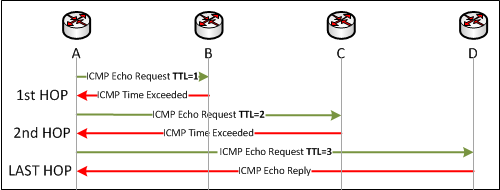
\includegraphics[width=0.7\textwidth, keepaspectratio]{figures/traceroute-works.png}
	\caption{A Traceroute útvonalfelderítés elve\protect\footnotemark}
	\label{fig:traceroute-works}
\end{figure}

\footnotetext{Forrás: \url{https://telconotes.wordpress.com/2013/02/08/how-traceroute-works/}}

Egy másik sokat használt mérőszoftver a ping, amely csak a célgéppel szemben tart fent elvárást, a közbülső gépekkel nem. Egy válaszkérő üzenetet küld, amelyre ha válasz érkezik akkor elérhetőnek számít a cél cím és a csomag körüljárási idejét is meg lehet állapítani.

Az eddig említett mérési elvek a hálózati eszközök szabványokban meghatározott működése alapján végeznek méréseket. A mérőrendszerben is alkalmazott iperf mérőszoftver viszont a cél címen telepített és futó példány segítségével képes csak a méréseket végrehajtani. Emiatt az üzemeltetése bonyolultabb, azonban információkban gazdag méréseket lehet végezni vele. Legfontosabb felhasználási funkciója a sávszélesség mérés.

\subsection{Passzív mérések}

Egyes esetekben szükségesek a vizsgálandó hálózatot nem terhelő vagy befolyásoló mérések. Ilyen esetekben passzív mérési eljárásokat alkalmaznak, melyek az áthaladó adatcsomagok vizsgálata alapján adnak visszajelzést a hálózat működéséről. Ilyen fajta méréseket főleg a hálózat üzemeltetői végeznek, mivel számukra egyszerű azokat végrehajtani a hálózati eszközök beállításával vagy az összekötő linkekre csatlakoztatott mérőeszközökkel. Egyik legelterjedtebb passzív hálózatmérési eljárás a Netflow, amelyet a Cisco fejlesztett ki, majd az IETF\footnote{Internet engineering task Force} is szabványosított. Működési alapelve, hogy a hálózati eszközökön az átmenő forgalmat egyes tulajdonságai alapján\footnote{Küldő/fogadó IP cím, küldő/fogadó port, használt protokoll, szolgáltatási osztály} folyamokba(flow) klasszifikálja, majd a generált forgalmuk historikus feljegyzésre kerül további elemzésre. 
%source/destination IP address, source/destination ports, protocol interface and class of service
% Netflow leírás: http://www.cisco.com/c/en/us/products/collateral/ios-nx-os-software/ios-netflow/prod_white_paper0900aecd80406232.html

\subsection{Hibrid mérések}

A korábban említett eljárások tulajdonságait ötvözik a hibrid hálózatmérési eljárások, melyek során mérési forgalmat generálnak a hálózatban, majd ezt passzív módon is megfigyelik. Ilyen módon egyszerre lehet információt kapni az egyes csomagok továbbítása során tapasztalt kezeléséről/életútjáról és a kapcsolat egészére vonatkozó tulajdonságokról. Ezzel a módszerrel lehet a legjobban megfigyelni a köztes elemek hatását a kapcsolat egészére.


\pagebreak

\subsection{További adatforrások}

Az Internet egészére vonatkozó mérések nehézségekkel néznek szembe annak mérete, folyamatos változása és tulajdonosi töredezettsége miatt. A következő \ref{internet-measurement} fejezetben ezen törekvéseket fogom bemutatni. Az alábbiakban ezek megértéséhez szolgáló további, az Internet tulajdonságait leíró adatforrásokat mutatok be.

Az előzőekben bemutatott IANA és a Regionális Internet Nyilvántartó szervezeteknek fontos feladata monitorozni az alájuk tartozó Internetes régiók működését. Az egyik legjobban bevált módszer a BGP protokoll hirdetéseinek a figyelése. Ezek a hirdetések az Autonóm Rendszerek közötti útvonalak helyen kiépítéséért felel. A BGP útvonalhirdetések megfigyelésére saját üzemeltetésű úgynevezett \mbox{Looking Glass\footnote{Angol jelentése tükör, lényegük hogy az Internet általuk látható felépítését közvetítik}} szervereket tartanak fent. 
Ezeknek a megfigyelési adatait pedig honlapjaikon\footnote{Példaként az RIPE honlapja: \url{https://atlas.ripe.net/landing/about/}} szabadon elérhetővé teszik, hogy további kutatók, üzemeltetők számára is átlátható legyen az Internet aktuális állapota.

Végső soron megemlítendőek még a WHOIS rendszerek, amelyek az egyes Internetes erőforrások tulajdonosairól adnak információkat, mint: IP címek, címtartományok, AS számok, DNS domének. Mindezen információforrások segítségével már komoly rálátással lehet bírni az Internetet alkotó Autonóm Rendszerekre.




%Looking Glass

%Cucc \cite{networkMeasure}.



%Internetes mérések (5-6 oldal): Aktív/Passzív, Looking Glass, traceroute, ping, iperf


\section{Internet felderítő projektek} \label{internet-measurement}

%(6 oldal): CAIDA, Archipelago és egyéb mérőrendszerek, PlanetLab, útvonal eltérítések esetei


Jelen fejezetben a legfontosabb Internet felderítését célzó szervezeteket és projekteket ismertetem, illetve megemlítem a legfontosabb ezeket felhasználó cikkeket.


\subsection{Internet elemző központ: CAIDA}

%\textbf{2-3 oldal kb}

A CAIDA (Center for Applied Internet Data Analysis)\footnote{\url{http://www.caida.org/home/}} egy kollaborációs együttműködése állami, kutatói és kereskedelmi szervezeteknek aminek célja az Internet üzemeltetésének, felügyeletének és fejlesztésének segítése. Alapvetően az alábbi három fő területre koncentrálódnak a szervezet munkakörei és projektjei:

\begin{itemize}
\item Kutatás és analizálás
%Research and Analysis	Analyze
\item Mérés és infrastruktúra
%Measurements and Infrastructure
\item Adat és eszközök.
%Data and Tools.
\end{itemize}

Munkájuk során az Internet egyes aspektusainak megismeréséhez modelleket készítenek, majd vizsgálják azok érvényességét, végül publikálják a talált összefüggéseket. Céljuk előremozdítani az Internet növekedésének problémamentességét. Ennek érdekében folyamatosan feltérképezik az Internet szerkezetét, amelyet a korábbi fejezetekben is bemutattam. Évente új \mbox{\glqq térképet \grqq} készítenek az Autonóm Rendszerek hálózatáról, mind az IPv4, mind az IPv6-os hálózatrészekről külön-külön. A \ref{fig:caida-poster} ábrán látható gráf pontjainak (AS) elhelyezése a földön is betöltött szélességi foka alapján (irány) és a rajta átmenő linkek száma alapján vannak elhelyezve (sugár, logaritmikusan ábrázolva).

\begin{figure}[!ht]
	\centering
	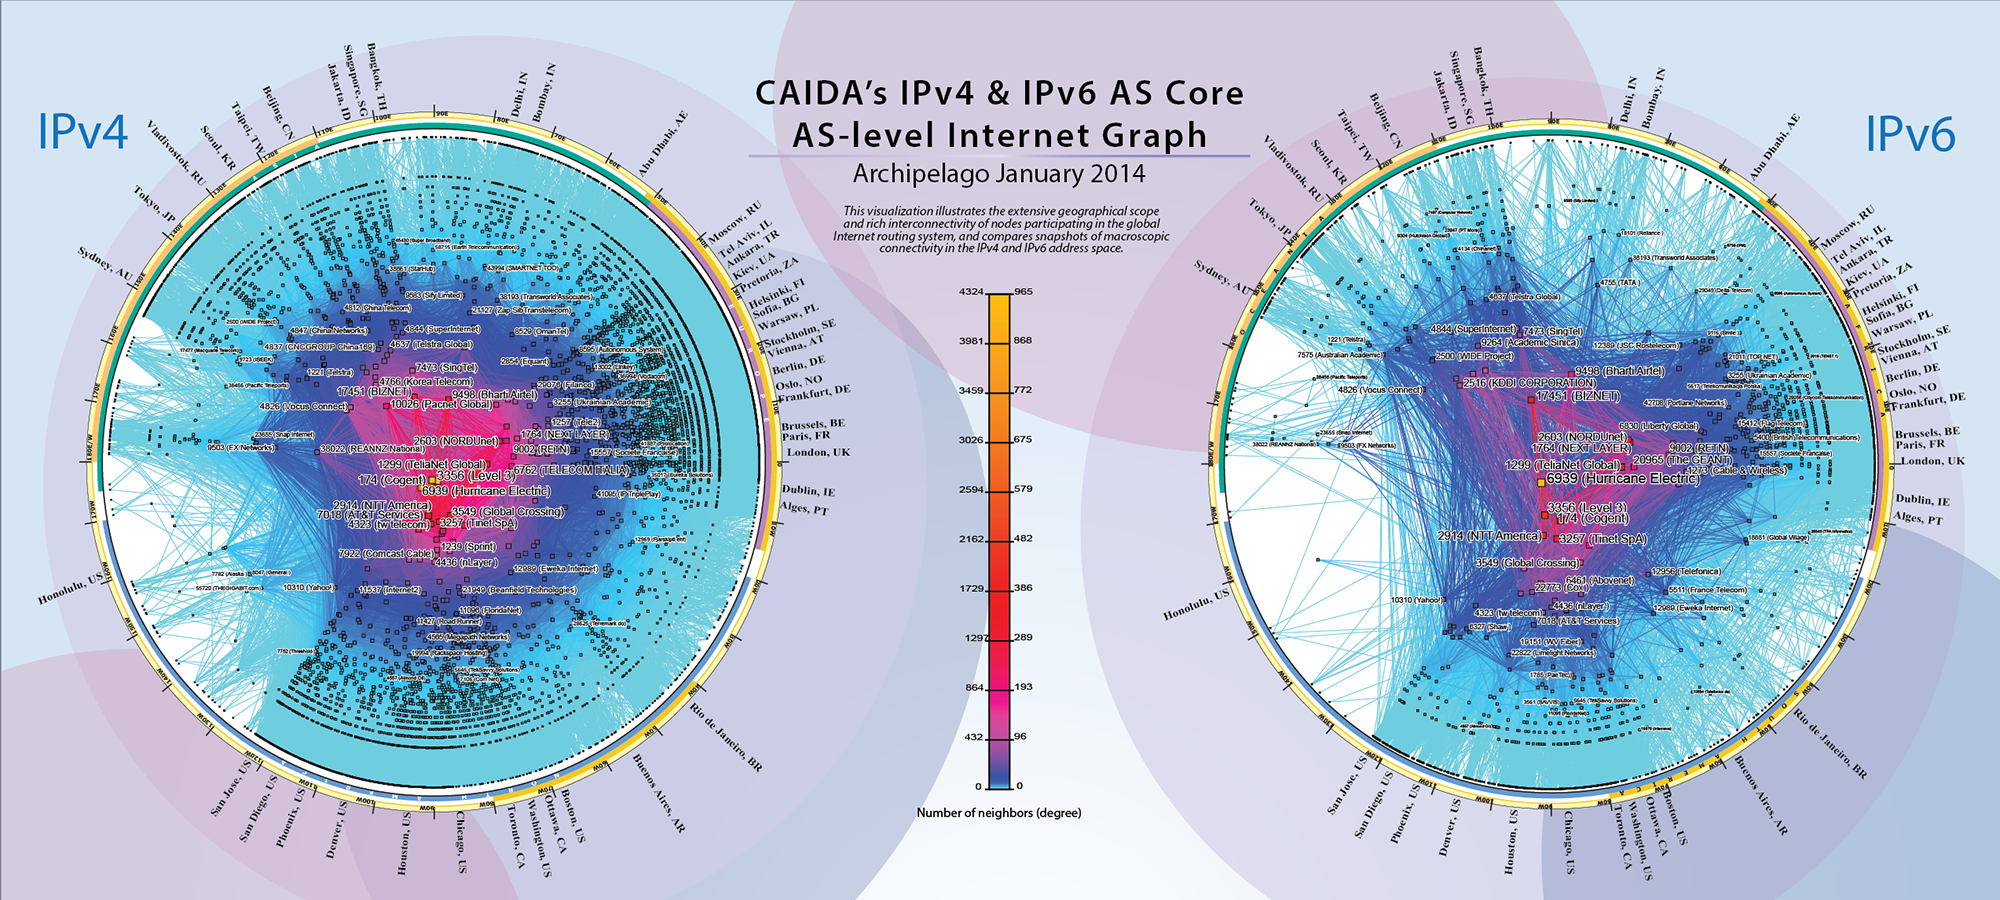
\includegraphics[width=0.9\textwidth, keepaspectratio]{figures/caida-poster.png}
	\caption{Az Internet AS gráfja 2014-ben}
	\label{fig:caida-poster}
\end{figure}

Az általános megfigyeléseken felül kutatásaik a kibervédelemre is kiterjednek. Céljuk az Internet helyes működése elleni tevékenységek felderítése és utólagos megértésük.


Ezen széles skálájú megfigyelésekhez kiterjedt mérési rendszereket üzemeltetnek a világ minden táján. Többek között begyűjtik az összes publikusan elérhető BGP útvonalhirdetéseket és a kooperáló szervezeteknél elhelyezkedő traceroute szerverekkel felméréseket végeznek a csomagtovábbítási viszonyokról az Internet egyes részeiben. Mindezeken felül pedig több Autonóm Rendszer hálózatában passzív méréseket is végeznek. Ennek a felhasználására egy példa az internetes háttérzaj mérése, ami az olyan adatcsomag küldések intenzitását mérik, amelyek olyan cél címekkel rendelkeznek ahol nem létezik fogadó számítógép. Az ilyen csomagok általában botnetek terjedési próbálkozásának a terméke.

Az említett adatforrások egy központi gyűjtő és organizáló rendszerbe, az ARK\footnote{Archipelago}-ba vannak csatornázva. A feldolgozás során rendkívül nagy hangsúly van fektetve a kinyert adatok hivatalosításán. Minden származtatott adatban meg vannak jelölve annak forrásai, valamint a különböző forrásokból származó azonos információk gondosan össze vannak vetve, ellenőrizve megbízhatóságukat.

%további tartalom majd innen: http://www.caida.org/home/about/progplan/progplan2014/
%% fél oldal kb eddig

%második oldal a 3 fő tématerületének a kifejtése, témánként fél oldal.

%Számunkra legfontosabb.. felsorolás a projektjeik közül

%%%%%%%%%%%%%%%%%%%%%%%%%%%%%%%%%%%%%%%%%%%%%%

\subsection{PlanetLab}

A PlanetLab konzorcium egyetemi, ipari és kormányzati intézmények együttműködő csoportja, amelyek erőforrásaikat megosztják kutatási céllal, így építik és fejlesztik a PlanetLab számítógépes hálózatát. A résztvevő szervezetek így hozzáférnek a sajátjuknál nagyobb hálózathoz. Ilyen módon a résztvevők kivételes lehetőséghez jutnak, hogy  nagyméretű hálózatokon és elosztott rendszereken tudjanak vizsgálatokat végezni.

A konzorciumot 2002-ben alapította 10 amerikai egyetem az Intel Research közreműködésével, kezdetben 100 számítógép-csomópont létrehozásával. A közösségi teszthálózat évről évre bővült újabb egyetemek és ipari kapcsolatok csatlakozásával. A PlanetLab 2004-ben több Amerikán kívüli szervezetet is befogadott többek között európából, brazíliából és ázsiából. Ebben az évben így már világméretűvé nőtt és több mint 400 számítógép csomóponttal rendelkezett. Napjainkban ez a szám már túllépte az ezret és az \ref{fig:planetlab} ábrán látható, hogy a föld minden táján megtalálhatóak a hálózatban résztvevő csomópontok.

A fejlesztett mérőrendszer is a PlanetLab hálózatát felhasználva végez méréseket az internet szerkezetére vonatkozóan.

\begin{figure}[!ht]
	\centering
	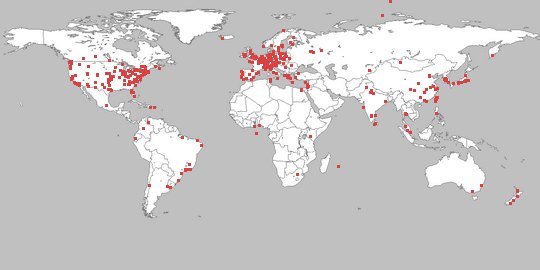
\includegraphics[width=0.65\textwidth, keepaspectratio]{figures/planetlab_worldmap.png}
	\caption{A PlanetLab teszthálózat csomópontjainak elhelyezkedése a világtérképen\label{fig:planetlab}}
\end{figure}

\subsection{M-Lab}
%2 oldal

Az előzőekben bemutatott PlanetLab és további piaci és kutatói szervezetek, többek között a Google, által alakított csoport, melynek célja az Internetes kapcsolatok végfelhasználói szemszögből való elemzése. Egyik legfontosabb célja a felhasználói élmény szűk keresztmetszetének a felderítése.

Begyűjtött adataik fontos része ilyen módon az önkéntes mérésekből származnak. Méréseket a weboldalukról, mobileszközről és telepített szoftverekkel lehet indítani. Minden adatuk nyilvánosan elérhető és letölthető. Több kutatási projektet is támogatnak mérési adataikkal. Naponta több mint 200 ezer tesztet futtatnak, melyek 750 TB adatot gyűjtöttek össze 2015-ig. 


%Elég nagy és működő félig üzleti szervezetnek tűnik. A Google is részese, gondolom ellenőrizni akarják hogy az ISP-k jól működnek-e. Egyik eszközük például külön kutatja, hogy mi a legszűkebb keresztmetszet az ügyfél kapcsolatában.
%Honlapjuk: http://www.measurementlab.net/
%Mobil mérésekkel is foglalkoznak, készítettek egy mobil applikációt ami adatokat gyűjt mérésekről. 2012 és 2013-ban kapott adatok elérhetőek: https://www.measurementlab.net/tools/mobiperf/

\subsection{SamKnows}
%1 oldal

Az Európai Unió és az amerikai FCC is felkarolta az egyetemi projektből kifejlődő SamKnows\footnote{\url{https://www.samknows.com/}} cég működését. Eredetileg a hétköznapi emberek könnyebb és objektív ISP választását segítette a projekt. Kezdetben önkéntesek végeztek méréseket a fejlesztett rendszerükön, hogy megállapítsák a szolgáltatójuk kapcsolatának minőségét. Nem csak sávszélesség mérésre alkalmas, de további hálózati paraméterek mellett a szolgáltatások diszkriminációját is figyeli. Olyan speciális adatcsomagokat használ a mérésekhez, amelyek HTTP, FTP, torrent, youtube, netflix, vagy VOIP\footnote{Voice Over IP - IP alapú hangkapcsolati protokoll} forgalmat szimulálnak. Ezen funkciói miatt rendkívül hasznos ellenőrzési eszköze lett a felügyeleti hatóságoknak. Folyamatosan fejlesztik a rendszerüket és riportokat készítenek a szolgáltatókról és működésükről.
%Az korábbi Internetsemlegességi vitáknál is felhasználták az így gyűjtött adatokat.
Mérési rendszerük támogatja a weboldalon keresztüli méréseket, mobil applikáción keresztüli méréseket és különböző telepíthető hardverelemeket is felhasznál, mint például a SamKnows Whitebox.

\begin{figure}[!ht]
	\centering
	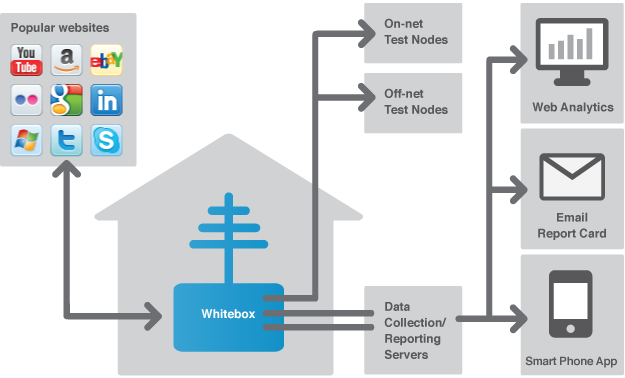
\includegraphics[width=0.45\textwidth, keepaspectratio]{figures/samknows-whitebox.png}
	\hspace{20pt}
	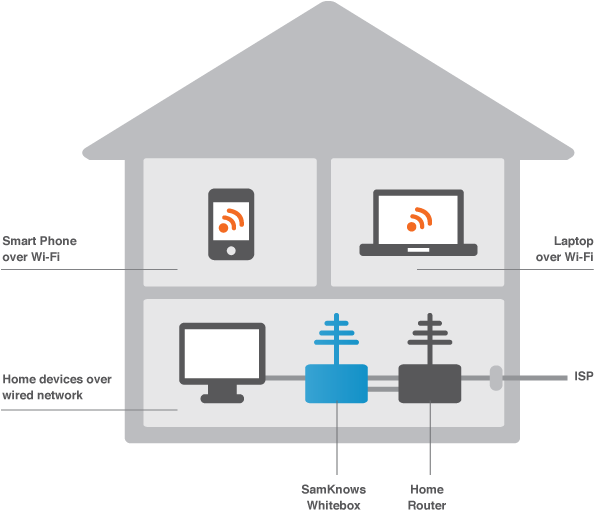
\includegraphics[width=0.45\textwidth, keepaspectratio]{figures/samknows-whitebox2.png}
		
	\caption{A SamKnows Whitebox méréseinek vázlata és elhelyezkedése a háztartásokban}
	\label{fig:samknows}
\end{figure}

A Whitebox készülékek működési elvét a \ref{fig:samknows} ábrák mutatják be, amely a korábban említett méréseket végzi el egy a háztartás hálózatába kötött eszköz segítségével. Az Európia Unió 2012-ben kérte fel a SamKnows céget a tagállamok interneteléréseinek a vizsgálatára. A tanulmány\footnote{\href{https://ec.europa.eu/digital-single-market/news/quality-broadband-services-eu-samknows-study-internet-speeds}{Quality of Broadband Services in the EU}} során 9467 háztartásba helyezték el a Whitebox készülékeket. A mérési adatok publikusan elérhetőek a \url{data.europa.eu} honlapról


\subsection{A DIMES mérési rendszer}
%1.5-2 oldal

2010 és 2013 között több egyetem bevonásával egy Izraeli kutatócsoport indította el a DIMES (Distributed Internet Measurement and Simulation) kutatóprojektet. Céljuk az Internet struktúrájának és topológiájának a megismerése volt, amelyet önkéntes módon segítenek további résztevők.
Az önkéntesek szerepe a geológiai diverzitás volt, amelynek segítségével több megfigyelési pontból lehet megvizsgálni az Internet szerkezetét.
Az elvégzett mérések egyszerű Ping és Traceroute mérésekből álltak, amelyek minimális erőforrásigényt támasztottak az önkéntesek gépein. A résztvevők cserébe személyre szabott jelentéseket kaptak az internetes kapcsolatuk minőségéről.

Kutatási eredményeik felhívták a figyelmet az Autonóm Rendszerek rendkívüli változatosságára és kapcsolataik nehezen felderíthetőségére. Egyik fontos megállapításuk a CAIDA akkori felméréseihez képest, hogy a Looking Glass szervereken keresztül elérhető BGP hirdetésekből hiányoznak az egyes AS-ek peering egyezményeikből fakadó összeköttetések.

A kutatási projekt aktivitása 2013 óta teljesen megszűnt, a hivatalos honlapjuk nincs karbantartva.

%Honlapja: http://www.netdimes.org/new/
%A DIMES honlapja gyakorlatilag nem működik, mindenféle hibákba ütközik (de legalább elérhető). A legutolsó hír rajta vagy bejegyzése 2013-ban íródott. Nem erléhetőek sajnos így az általuk elért adat sem, sem az infók róla :(
%A publikációjukból tudunk legjobban kiindulni: link (2000 és 2013 közöttiek)
%A saját mérési adataik elérhetőek: link
%Lehet érdemes felvenni velük a kontaktot, hogy külsős fél mennyire tudná most futtatni?
%Email: support@netdimes.org
%A projekt résztvevői: link
%A projekt fóruma: link
%A fórumon van egy “friss” szál ahol megbeszélik, hogy ez egy halott projekt (link).
%Ebben a beszélgetésben egy lényegretörő hozzászólás:
%Since I found the project I've now gotten rid of all Windows machines, and the Linux version never worked anyway. I can't run the agent either way.

\subsection{Kisebb Internet mérő projektek}

A fentiekben felsoroltakon kívül még számos kisebb internet mérést célzó projekt létezik még melyek közül a továbbiakban kettőt emelek ki.

\subsubsection*{Az IRL mérési rendszer}
 
 
Egyetemi projektként\footnote{\url{http://irl.cs.tamu.edu/projects/sampling/}} kutatásuk középpontjában a teljes Internetre vonatkozó mérések hatékonyságának a növelése állt. Új eljárásokat fejlesztettek ki, melyekkel nem a bevett elárasztásos módon derítik fel az egyes hálózati tartományokat. Utóbbi publikációjukban\cite{irl-measure} pedig a hálózatban résztvevő eszközök operációs rendszerét állapították meg.
 

%Sampling Internet structure and its service availability have always been important issues in Internet research. This project aims to develop mechanisms for discovering available services in the Internet using scalable end-to-end measurements, facilitate delay sampling between arbitrary hosts using the existing DNS infrastructure, perform more accurate bandwidth estimation, and build router-level maps of the Internet using non-intrusive traceroute to known destinations. We are also working on techniques for fingerprinting OS and server implementations using low-overhead end-to-end methods.


\subsubsection*{Az iPlane mérési rendszer}
 


Diploma munkaként született, majd kutatási projektté fejlődött az iPlane\footnote{\url{http://iplane.cs.washington.edu/}}, melynek fő célja az internetes útvonalak QoS becslése és akár predikciója. Kimutatásaikat a PlanetLab gépeken és további publikus Traceroute szervereken futtatott útvonal felderítő mérések alapján végezték. Céljuk a felhalmozott adatok felhasználása későbbi szolgáltatások minőségének javítására.Elemzéseik fontos része, hogy a felderített útvonalaknak a rész szakaszaira becsülnek paramétereket, így még nem mért útvonalak viselkedésére is tudnak becslést szolgáltatni. Ezt a becslést pedig Peer-to-peer és Voice-Over-IP alkalmazások működésének javítására használták.

%Alapvetően egy mellék képessége az internetes utak  emgfigyelése, mérése. A lényege az internetes útvonalak QoS becslése, jóslása a korábbi mérésekből, valamint ennek a felahsználása a felsőbb szolgáltatások javítására. Szintén PlanetLab os gépeket használ, valamint további publikus traceroute szervereket a mérések elvégzésére.
%Rengeteg traceroute mérést végeznek, még napjainkban is, ezek elvileg elérhetőek bárki által. (Akár mi is hasznosíthatnánk?)
%Nem elérhető a rendszerük forrása, kicsit homályos a működése (valószínűleg a publikációjukból meg lehetne ismerni).
%Az iPlane egy Diploma  munka eredménye, itt van maga a dimploma: link

%iPlane is a scalable service providing accurate predictions of Internet path performance for emerging overlay services. Unlike the more common black box latency prediction techniques in use today, iPlane builds a structural model of the Internet. We construct an annotated map of the Internet and predict end-to-end performance by composing measured performance of segments of known Internet paths. This method allows us to accurately and efficiently predict latency, bandwidth, capacity and loss rates between arbitrary Internet hosts. We have studied the feasibility and utility of the iPlane service by applying it to several representative overlay services in use today: content distribution, swarming peer-to-peer filesharing, and voice-over-IP. In each case, we observe that using iPlane's predictions leads to a significant improvement in end user performance. 
%Internet felderítése (6 oldal): CAIDA, Archipelago és egyéb mérőrendszerek, PlanetLab

%------------------------------------------------
%Mérőrendszer felépítése (13-15 oldal):

\chapter{Automatizált Internet mérő rendszer}
%(13-15 oldal): 

Jelen fejezet mutatja be az elkészült automatizált mérési rendszert, annak felépítését és működési elvét.

\section{Mérési elrendezés}
%(5 oldal): traceroute, iperf, mérési forgatókönyvek, PlanetLab

A felhőben vagy kliensen futó szoftver óránként felméri a PlanetLab hálózat gépeinek elérhetőségét és a kapott adatokat, statisztikákat eltárolja az adatbázisában. A PlanetLab hálózatában ugyanis elméleti szinten 1200 körüli végpont van, azonban ezeknek nagy százaléka elérhetetlen. A külön lépésben való feltérképezéssel rengeteg sikertelen kapcsolódást kerül el a mérőrendszer. A csatlakozásra képes célgépekre SSH kapcsolaton keresztül felcsatlakozik. Az egyes mérési forgatókönyveknek megfelelően parancssorozatokat futtat, majd azok eredményeit adatbázisban tárolja.
A nyers mérési eredmények, mint például a traceroute kimenet, később további feldolgozási lépéseken mennek keresztül. Végül az egyes kimutatásokhoz további statisztikák készülnek.
Az alábbiakban ezen lépések kerülnek részletesebb bemutatásra.

\subsection{A méréshez használt hálózat}

Az Interneten végzett mérésekhez szükséges a hálózatok különböző pontjain végezni méréseket. Egyes mérésekhez elegendő egy végpontból elvégezni a méréseket, azonban az csak lokális képet ad vissza, így torzítja az egész Internetről alkotott képet. A mérési rendszer üzemeltetéséhez ezért szükséges volt hozzáférést szerezni további a hálózatban résztvevő csomóponthoz. Így minél több résztvevő szolgáltat mérési adatokat, annál egységesebb képet tudunk kapni a kinyert adatokból. Az előző \ref{internet-measurement} szekcióban bemutatott hasonló mérési rendszerek szintén kiterjedt mérési hálózattal rendelkeztek. A PlanetLab hálózata kézenfekvő megoldás az Internetes mérések végzéséhez. Kiterjedésének nagysága biztosítja a mérés reprezentativitását, valamint megbízhatósága garantálja a mérések sikerességét.

A mérési rendszer azért jöhetett létre, mert a Budapesti Műszaki és Gazdaságtudományi Egyetem, ahol a Diplomamunkámat végeztem, résztvevője a PlanetLab szervezetnek. A részvételhez szükséges volt a megfelelő kapcsolattartó személyek kinevezése és a hálózat számára elérhetővé tenni két szerver gépet, amelyek megfelelnek a követelményeknek. A redundancia érdekében kötelező a két független gép. A hardveres paramétereken felül feltétel volt a szervezet által fejlesztett Linux disztribúció telepítése, amely fel van készítve a megfelelő virtualizáció támogatására. A tudományos mérések izolációjához szükséges a virtualizáció, így ha a szervezet egy résztvevője hibás programot futtat, az nem lesz kihatással a többiek által végzett mérésekre. A hozzáférések biztonságát a kötelező publikus-privát kulcsok használatával garantálják. Miután a mérésekhez generált publikus kulcs feltöltésre került a szervezet központi honlapjára, a mérésekhez már fel is lehetett használni.

A hálózatban elérhető gépekkel kapcsolatban fontos szempont továbbá, hogy hiába van elkülönített virtualizált környezet a résztvevők számára, azokon nem lehet tárolni adatokat. Bármikor felszólítás nélkül új virtualizált környezetet osztanak ki a felhasználók számára. Ezzel biztosítják a szerverek elérhetőségét és a folyamatos tisztulását. A Mérési rendszer készítésekor részben ezért volt szükséges az egyes mérési eredmények azonnali tárolása adatbázisban.

\subsection{Csatlakozás a hálózat számítógépeihez}

A mérések elvégzéséhez szükséges volt a PlanetLab hálózatának gépeihez való automatizált csatlakozás és parancs végrehajtás. A hálózatában résztvevő számítógépek listáját egy központi célgép szolgáltatja.

A mérések elvégzéséhez és feldolgozásához egységesen Python programozási nyelven megírt szkriptek lettek használva. A nyelv rugalmassága, támogatottsága és az elérhető könyvtárak bősége tette alkalmassá a gyors fejlesztésre. 
A méréseket végző program a Paramiko\cite{paramiko} könyvtárat használja az ssh kapcsolatok felépítéséhez és menedzseléséhez. A mérési kísérletek sok esetben hiúsultak meg különböző hibák, vagy a célszámítógép elérhetetlensége miatt, ezért ezen esetek kezelése fontos szempont volt a fejlesztés során. A \ref{fig:statistics} ábrákon látható statisztikák az első mérések adataiból készültek. A mérések óránként lettek elvégezve, lefutásonként 1354 csomóponthoz téve csatlakozási kísérletet. A vezérlő számítógép nem állandóan futott, így egy hónapban csak 23 nap készültek mérések, átlagosan 15 alkalommal.


\begin{figure}[h!]
\begin{center}
    \subfigure[Csatlakozási kísérletek eredményessége]{\label{fig:succeed}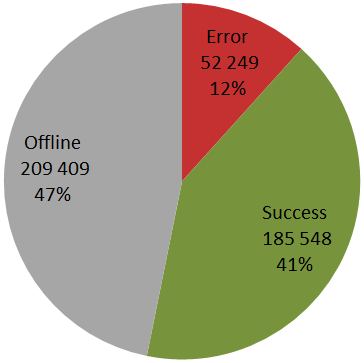
\includegraphics[scale=0.4]{figures/succeed.png}}
    \hspace{10mm}
    \subfigure[Hibák okai]{\label{fig:errors}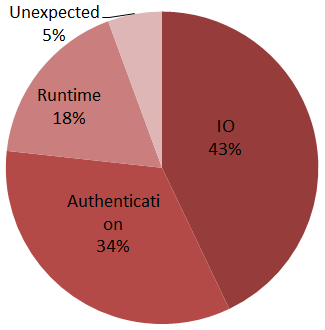
\includegraphics[scale=0.45]{figures/err.png}}
	\caption{Statisztikák\label{fig:statistics}}
\end{center}
\end{figure}

\subsection{Időzített mérési forgatókönyvek}
Az iperf mérések implementálásához új eljárás kidolgozására volt szükség a mérést menedzselő szoftverben. A korábbi traceroute mérések egyetlen parancs távoli futtatásából álltak, amelyek futási eredményét tároltuk el mérési eredményként. Az iperf és más sávszélesség mérő szoftverek működéséhez azonban szükséges mind egy adatcsomagokat küldő és egy adatcsomagokat fogadó példány futtatása a két különböző távoli gépen. Ennek lebonyolításához a mérést lebonyolító programnak több szálon kell futnia, a két távoli kódfuttatást egyszerre kell végeznie. Először az adatcsomagok fogadását (szerver oldal) végző programot kell elindítani, majd csak ezt követően lehet csak a mérést megkezdeni az adatcsomagokat küldő program (kliens oldal) elindításával. A mérést követően a szervert pedig le kell állítani. Ez a szituáció tovább bonyolódik, ha két sávszélesség mérést párhuzamosan szeretnénk végezni. Ez egy fennálló igény, mivel a későbbiekben az MPTCP\footnote{Multipath Transfer Protocol: Több párhuzamos TCP adatfolyamon végez kommunikációt a felsőbb rétegek felé egyetlen TCP kapcsolatot emulálva.} protokoll lehetséges viselkedését is vizsgálni szeretnénk.

Ezeket a lépéseket általánosítva olyan mérési forgatókönyvek létrehozását támogatja már a mérési rendszer, amely bármilyen távoli parancsok időzített futtatását garantálja. Ennek kialakítása a lehető legrugalmasabbra lett tervezve, amelynek működését a függelékben található példakód mutatja be. A kód egyszerűségének ellenére a mérés teljesen menedzselt, bármilyen hiba keletkezése le van kezelve és megfelelően naplózva és a mérési eredményben jelezve van. Garantálva van a helyes időzítés, a párhuzamos futás és a helyes leállás.

%A mérési forgatókönyvek rendkívül hasznosak, segítségükkel új mérések implementálása kényelmes és gyors.


\section{Geolokációs és AS információk}
Az internetes útvonalakat alkotó IP címekről több információt is tud kinyerni a mérési rendszer. Ilyen az ip címhez tartozó autonóm rendszer azonosítója, valamint a becsült geolokációs elhelyezkedése. Ezekhez Python szkriptek lettek készítve, amelyek ingyenes online szolgáltatásokat vesznek igénybe. A nagy feldolgozandó adatmennyiség és a sokszor lassú kapcsolódás miatt helyi gyorsítótár alkalmazása volt szükséges.

\section{Middlebox felderítés}
A tanszéken végzett Internetes kutatásokhoz hozzáadott értéket jelentett a mérési rendszer. A kutatás középpontjában napjaink egyik Internetes trendje az úgynevezett Middlebox-ok voltak. Ez egy általános fogalom minden olyan hálózati eszközre vonatkozóan, amely beavatkozik és manipulálja a rajta átmenő forgalmat. Ilyen lehet a hagyományos tűzfal vagy terheléselosztó, de manapság újabb és újabb célra használják fel, néha beavatkozva a végpontok közötti kapcsolatba. Ez az Internet alapjait jelentő protokollok működésére akár nem kívánt hatással is lehet, ezért fontos kutatási téma napjainkban.

A kutatáshoz való hozzájárulása a mérési rendszernek az interneten küldött csomagok TTL mezőjének a manipulációját vizsgálta. Egy célgépen a tcpdump nevű alkalmazást volt elindítva olyan beállításokkal, hogy csak a mérésben résztvevő csomagokat vizsgálja. A PlanetLab hálózat elérhető gépein pedig speciálisan elkészített csomagok voltak küldve a célgép felé a maximális 250-es TTL mezővel. A vizsgálat a Middlebox-ok TTL manipulációját figyelte a különböző csomagtípusokra vonatkozóan.

Három csomagtípus manipulációja volt vizsgálva:

\begin{itemize}
\item \textbf{ICMP Ping request} Hagyományos ping üzenet kérési csomagja
\item \textbf{TCP SYN port:22} TCP kapcsolatfelépítési csomag a 22-es portra, amely az ssh kapcsolatok fogadására szolgál
\item \textbf{TCP SYN port:80} TCP kapcsolatfelépítési csomag a 80-as portra, amely a http kapcsolatok fogadására szolgál
\end{itemize}

\pagebreak

A felhasznált parancsok a következők voltak:

\begin{lstlisting}[language=bash]
  # Celgepen futtatott parancs ICMP csomagok fogadasara
  sudo tcpdump -vnn -i eth0 icmp[icmptype] == 8 and dst host $ip
  # PlanetLab gepekrol kuldott ICMP csomagok parancsa
  ping -c 1 -t 250 $ip
  
  # A celgepen futtatott parancs TCP SYN csomagok fogadasara
  sudo tcpdump -vnn -i eth0 dst host $ip and "tcp[tcpflags] & (tcp-syn) != 0"
  # A PlanetLab gepeirol kuldott TCP csomagok parancsa
  nmap -v --ttl 250 --max-retries 1 -PS -p 80 $ip
  nmap -v --ttl 250 --max-retries 1 -PS -p 22 $ip
\end{lstlisting}


A mérés egy korábbi tanulmányt\cite{middlebox} vett alapul a felderítéshez. Az Internetes útvonalakon található, ttl mezőt manipuláló Middlebox-ok jelenlétét kimutatta a mérés. A mérés 75 szerverről küldött csomagok alapján lett elkészítve, mindegyik csomagtípusból egyet küldve a célgép felé, kivéve a 80-as portra küldöttek, amelyekből 3 csomag lett küldve gépenként.


\begin{figure}[!ht]
	\centering
	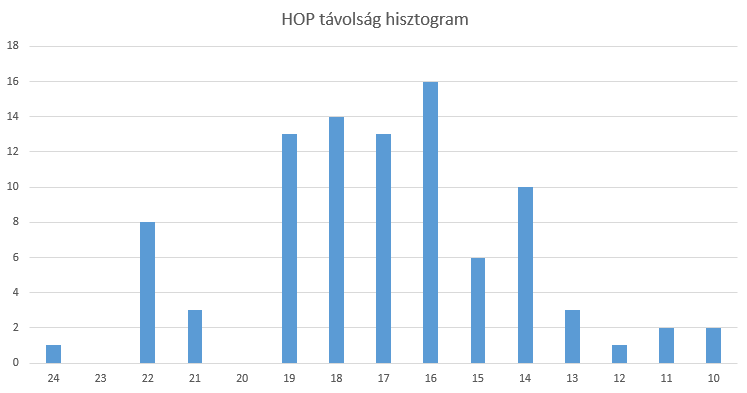
\includegraphics[width=0.5\textwidth, keepaspectratio]{figures/hop-hist.png}
	\caption{Az eredeti HOP távolsága a mért útvonalaknak}
	\label{fig:hop-hist}
\end{figure}


\begin{figure}[!ht]
	\centering
	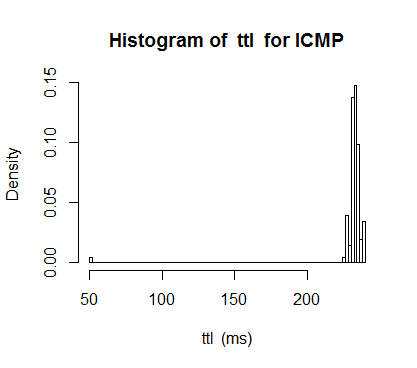
\includegraphics[width=0.3\textwidth, keepaspectratio]{figures/hist-ttl-icmp.png}
	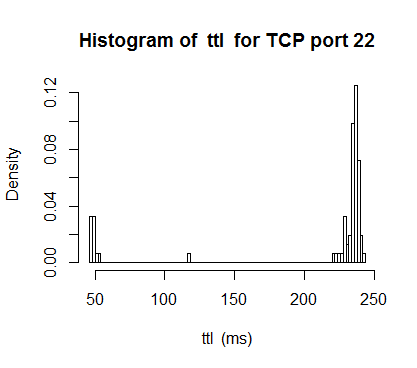
\includegraphics[width=0.3\textwidth, keepaspectratio]{figures/ttl-hist-22.png}
	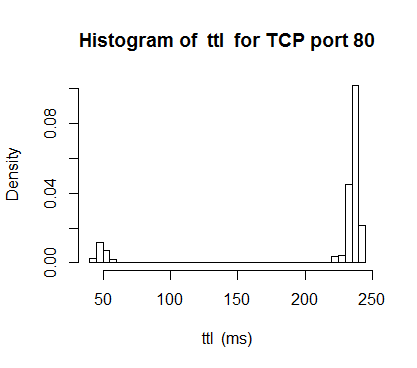
\includegraphics[width=0.3\textwidth, keepaspectratio]{figures/ttl-hist-port80.png}
	\caption{A fogadott csomagok TTL értékeinek előfordulási sűrűsége}
	\label{fig:ttl-hist}
\end{figure}

A \ref{fig:ttl-hist} ábrán látható, hogy az eredetileg 250-es TTL mezővel küldött csomagok egy része fogadáskor már egy közbülső elem által manipulálva lett. A manipuláció abból következtethető, hogy az útvonalak hosszúsága normális eloszlást követ, ahogy a \ref{fig:hop-hist} valamint függetlennek kellene lennie a csomag típusától.

Az ICMP csomagok ábráján egyetlen csomag érkezett vélhetően módosított TTL mezővel, későbbi ellenőrzéskor azonban kiderült, egy nem a mérésben résztvevő gép küldte. A méréshez használt csomagszűrő minden Ping requestet átengedett, azonban a mérés ideje alatt a colorado-i egyetem egyik szervere is küldött ilyen csomagot. Ilyen módon kimondhatjuk, hogy az ICMP csomagok TTL mezője nem megy keresztül módosításon. Ezzel szemben a TCP csomagok, amelyeket vizsgáltunk az esetek több mint 10\%-ában módosításon estek keresztül. A 80-as portra küldöttek 11\%-a, míg a 22-es portra küldöttek 15\%-a. Itt megjegyzendő, hogy nem következetes az útvonalakon közbeiktatott manipuláció. Egyes útvonalakon csak a 22-es portra küldött csomagok lettek változtatva, másokon csak a 80-as portra küldöttek és természetesen legtöbb esetben mindkettő. Ezen felül a 80-as portra küldött 3 csomagból, manipuláció esetén a legtöbb esetben egyszerre voltak csökkentett TTL mezőjűek és érintetlenek is.

Ez a mérés jól mutatja be a mérési rendszerben rejlő potenciált. A PlanetLab hálózatnak köszönhetően, az Internetre reprezentatív eredmények jöhetnek létre a gyorsan összeállítható mérési forgatókönyveknek hála.
%Mérési elrendezés (5 oldal): traceroute, iperf, mérési forgatókönyvek, PlanetLab


\section{Fejlesztési megfontolások}
%(8-10 oldal): python, mongodb, logolás, email küldés, weboldal, hibák függetlenítése, megbízhatóságnövelő megfontolások


\subsection{MongoDB adatbázis használata}
Először SQLite adatbázis volt használva a mérési eredmények tárolására. Az SQL lekérdezési nyelvet széleskörű ismerete miatt lett használva, valamint a Python programozási környezetből való kényelmes használta miatt. Az adatbázis egyszerű fájlként van tárolva, így könnyebben kezelhető. A fejlesztés közben sűrűn változó struktúrájú adatok tárolásár azonban nem volt megfelelő. Egy új mérési attribútum bevezetésekor új adattáblát kellett létrehozni, a régi adatokat pedig megfelelően importálni. A felmerülő adatkonverziók feleslegesen vettek el időt. Ezen felül az adatok feldolgozása is erőforrás igényes volt, mivel a komplexebb adatfeldolgozási lépések Python szkripteken futottak amelyek többször fordultak újra az SQLite adatbázishoz.

Ezen problémák miatt más adatbázis megoldások lettek felmérve, amelyek jobban illeszkedhetnek majd a rendszerek igényeihez. A relációs adatbázisokkal szembe a dokumentum alapú adatbázisok nem rendelkeznek szigorú adatstruktúrákkal. Egy kollekcióban (az adattáblákhoz hasonló elem) többféle felépítésű adatelem is elhelyezkedhet. Egy hibás mérés adateleme például csak kevéssel különbözik a többitől. Ezek könnyen kezelhetően együtt tudnak élni egy ilyen dokumentum alapú adatbázisban, míg komplex relációs táblák kialakítása lett volna szükséges SQL esetében. Végül a MongoDB lett kiválasztva, a széleskörű adatfeldolgozási támogatása miatt. Egyes komplexebb feldolgozási lépéseket akár azonnal az adatbázisban el lehet végezni, a többfokozatú adataggregálási rendszerének és a JavaScript alapú map-reduce eljárásnak hála.

A választás meghozta eredményét, mivel felgyorsul az új adatfeldolgozások fejlesztése, valamint a régebbi struktúrájú mérések az újakkal könnyen együtt kezelhetővé váltak.

%%%%%%%%%%%%%%%%%%%%%%%%%%%%%%%%%%%%%%%%%%%%%%%%%
% Címszavakban a tartalom:
%rugalmas adatstruktúrák
%fejlesztés közbeni átmeneti állapotok jó kezelése
%Aggregálási képességek hangsúlyozása
%(komplex lekérdezése)


\subsection{Megbízhatósági törekvések}
A mérési rendszer úgy lett kialakítva, hogy bizonytalan körülmények között is megfelelően működjön. A PlanetLab hálózatában rendkívül sokféle számítógép található, amelyek karbantartása sok esetben nem megfelelő. Korábban olyanra is akadt példa, hogy egy PlanetLab-os számítógép rendellenes viselkedése leállította az egész mérési folyamatot. Az ehhez hasonló hibák elkerülésére valamint a hibák minél hamarabbi észlelésére nagy figyelem lett fordítva a mérési rendszer fejlesztésekor.

\subsubsection*{Hibalehetőségek függetlenítése}
A mérés egy folyamatos ciklusból áll: A PlanetLab gépeit megpróbálja elérni, azokon a megfelelő méréseket elvégezni, végül eltárolni az eredményeket, majd egy újabb géppel folytatni a mérést.
Korábban egy hiba fenntarthatta az egész mérést. Ennek elkerülése miatt két programszálra lett bontva a folyamat: Egy központi program folyamatosan iterál a PlanetLab gépein és egy újabb független programot indít a mérendő gép címét paraméterként megadva. A hívott program bármilyen hibába ütközik arról értesül a főprogram, de nem tudja leállásra kényszeríteni azt. Az alprogram futásának pedig egy félperces maximálisan megengedett időablaka van, amelyet ha meghalad automatikusan leállításra kerül és egy újabb méréssel folytatódik a ciklus.

\subsubsection*{Maximálisan megengedett időkeret elve}
Az maximálisan megengedett időkeret elvét több másik folyamatra is bevezettem. A mérés során ha bármely lépése a folyamatnak időkorlátba ütközik a hiba oka fel lesz tüntetve a mérésről készült jelentésben. Ilyen módon könnyen kideríthető a hiba oka.

\subsection*{Hibanaplók készítése}
A fejlesztés kezdeti szakaszában ha hiba fordult elő a kódban az viszonylag hamar kiderült és a fejlesztőkörnyezetben kényelmes eszközök álltak rendelkezésre, hogy a kiderüljön a hiba oka. Később amikor a mérés folyamatosan futott nagyban feltartotta a megoldását, hogy a hiba egyetlen jelensége az volt, hogy nem került mentésre egy újabb sikeres (vagy akár sikertelen) mérés sem. Ennek megoldására a mérésnek szinte miden szintjén be lett vezetve a hibanapló írása. Így a mérés állapota és az esetleges hibák forrásai egyből elérhetővé váltak. A felhős platformon pedig a hibanaplók akár a weboldalon egyből megtekinthetővé váltak.

\subsubsection*{Felmerülő hibák kategorizálása, előfordulásuk monitorozása}
Mint korábban említettem a PlanetLab hálózatán sok nem karbantartott gép is jelen van, emiatt a hivatalosan elérhető 1030 gépből átlagosan csak 400 elérhető ping paranccsal, amelyek közül átlagosan csak 200-hoz lehet sikeresen ssh kapcsolatot felépíteni és parancsot futtatni. A géppark állapotáról ezért óránként egy felmérés készül, amely a PlanetLab gépeihez csatlakozni próbál és a problémamentes gépeket nyilvántartja, hogy ne kelljen feleslegesen csatlakozási kísérletet végezni a hibás gépekhez. Ez az eljárás nagyban felgyorsította a sikeres mérések begyűjtését.

A csatlakozási és parancsfuttatási hibák a felmérés során kategorizálásra kerülnek és későbbi statisztikák számára tárolódnak. Így nyomon követhető a PlanetLab hálózatán elérhető gépek tényleges elérhetősége/használhatósága.
A mérési rendszer honlapján ezek a friss statisztikák szintén elérhetően, így könnyen felmérhetjük a tömeges hibák okait. Ilyenre volt példa amikor a BME által üzemeltetett PlanetLab gépek leálltak és a PlanetLab megszüntette a hálózatukban elérhető gépekre való csatlakozási engedélyünket. Egy új hibakategória jelent meg a felmérési statisztikákban amely hirtelen sok gépet tett elérhetetlenné (bár nem mindet).

%Fejlesztési megfontolások (8-10 oldal): python, mongodb, logolás, email küldés, weboldal, hibák függetlenítése, megbízhatóságnövelő megfontolások

%------------------------------------------------
%Mérési eredmények áttekintése (12-15 oldal):

\chapter{Mérési eredmények}
%%%%%%%%%%%%%%%%%%%%%%%%%%%%%%%%%%%%%%%%%%%%%%%%%
%(12-15 oldal)



%\section{Mérési eredmények}
%(7-10 oldal): kinyert mérések tartalma(delay, jitter, link, AS info, Geolocation), mérések mennyisége, mérések minősége

\section{Létrehozott adatbázis bemutatása}
Jelen fejezet bemutatja a létrehozott adatbázis fontosabb adathalmazait, amelyek további elemzések alapját képezi.

\subsection*{Éllista}
A legfontosabb eredmény az internetes útvonalakat alkotó gépek közötti kapcsolatokról szolgáltat mérési eredményeket. Az objektum amelyről a mérés készült egy internetes link, a kinyert információk a következők:

\begin{itemize}
\item \textbf{delay:} Késleltetés a két gép közötti kapcsolaton (két gép közötti elméleti rtt)
\item \textbf{rtt:} A from számítógéphez végzett körülfordulási idő a mérést végző measurer\_ip számítógéptől
\item \textbf{time:} A mérés időpontja
\item \textbf{jitter:} Késleltetés ingadozás a két számítógép között
\item \textbf{measurer\_ip:} A mérést végző számítógép (ahol a traceroute parancs fut)
\item \textbf{target\_ip:} Az útvonalmérés célpontja
\item \textbf{to:} A linkek a mérést végző számítógéptől távolabbi csomópontjának információi: city, country, longitude, latitude, ip, asn
\item \textbf{from:} A linknek a mérést végző számítógéphez közelebbi csomópontjának információi: city, country, longitude, latitude, ip, asn
\end{itemize}



Az elkészült mérési rendszernek ez az adat kollekció\footnote{A MongoDB adatbázisban táblák helyett kollekciókban tárolódnak az adatbejegyzések} az egyik legfontosabb eredménye. A Traceroute parancs futtatásának kimenetéből lett feldolgozva\cite{traceParse} és további adatmezőkkel felgazdagítva.

\begin{figure}[h!]
	\centering
	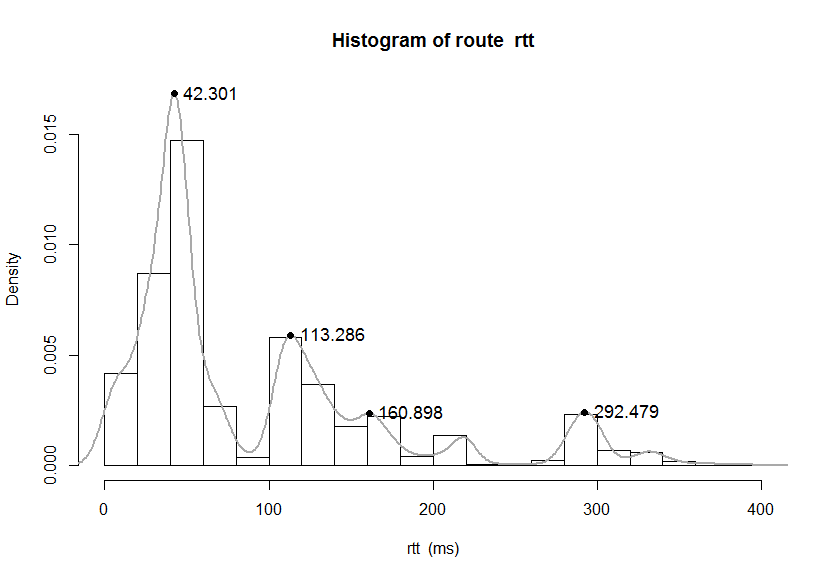
\includegraphics[width=0.95\textwidth, keepaspectratio]{figures/route_rtt_hist_max.png}
	\caption{Két végpont közötti késleltetés eloszlása}
	\label{fig:rtt-hist}
\end{figure}

A \ref{fig:rtt-hist} ábrán az egyik legalapvetőbb kimutatás látható, a késleltetések eloszlását a PlanetLab gépe között. Megfigyelhető az eloszlás lecsengése 350 milliszekundum felett, azonban a kimutatásból le lett vágva az rtt értékek felső 0.5\%-a. Ezek a mérések az esetek legnagyobb részében ideiglenes hálózati problémák alatt készültek, amelyek nem reprezentatívak a linkek tényleges tulajdonságaira vonatkozóan.

Az eloszlás első csúcsának elkülönülése a többitől az Internetet alkotó gráf útvonalainak a valós világhon alapuló tulajdonsága határozza meg. A mérési csomópontok túlnyomó része Európán vagy Amerikán belüliek, ezt magyarázza a 42 milliszekundum körüli első csúcs. Amint viszont egy kontinenseket átívelő linket érint a mérés, legalább 70 milliszekundumos késleltetés hozzáadódik az addigiakhoz, így adva a 113 milliszekundum körüli újabb csúcsot. A 70 milliszekundumos késleltetést a London-New York\footnote{Forrás: \href{https://wondernetwork.com/pings/New+York/London}{wondernetwork.com}} közötti tipikus késleltetés alapján lett figyelembe véve. A további késleltetés csúcsok további kontinensek közötti késleltetések alapján származtathatóak. Az hasonló kimutatások jól prezentálják az Internetnek a valós világunkhoz való szoros kapcsolatát.

Az rtt-ből származtatott delay adat az Internetet alkotó linkek és azok megfigyelhetőségére nyújt betekintést. Az útvonalakon lévő hálózati eszközök eltérő módon válaszolnak a lejárt TTL mezőjű adatcsomagokra, amelyeket a traceroute használ. Ennek legegyértelműbb bizonyítéka a delay adatsor kvantiliseinek értékei:

\renewcommand{\arraystretch}{1.3}
\begin{table}[ht]
	\centering
	\caption{A delay adatsor kvantilisei}
	\hspace{2mm}
	\begin{tabular}{ | c | c | c | c | c |}
	\hline
0\% & 25\% & 50\% & 75\% & 100\% \\ \hline
-2217.682 & -0.188 & 0.631 & 6.775 & 2323.324 \\ 
\hline
	\end{tabular}
	\label{tab:delay_kvant}
\end{table}

A \ref{tab:delay_kvant} táblázatból az olvasható le, hogy a delay értékeknek legalább 25\%-a negatív értékű és széles tartományon -2 szekundumtól +2 szekundumig terjed. A meglepően nagy arányban előforduló negatív értékek magyarázata az, hogy míg egy hálózati eszköz képességeinek megfelelően azonnal visszaküldi a lejárt TTL mezőjű csomagokat, addig egyes eszközök ezt késleltetve teszik meg.
Az adatsor eredeti hisztogramja nincs bemutatva, mivel egyetlen csúcs látszódna csak az origó környékén, a túlságosan szélsőséges értékek miatt.

\begin{figure}[h!]
	\centering
	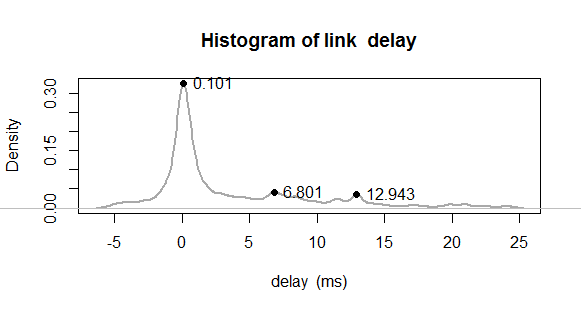
\includegraphics[width=0.95\textwidth, keepaspectratio]{figures/link-delay-dist.png}
	\caption{Két végpont közötti késleltetés eloszlása}
	\label{fig:link-delay}
\end{figure}

Az adatsornak ezért a két szélsőséges 5 percentilisét levágva készítettem el a valószínűségi változójának a sűrűségfüggvényét. Annak ellenére, hogy a linkekre becsült késleltetések többnyire 0,1 milliszekundum körül helyezkednek el az átlaguk 6,12 milliszekundum.

\pagebreak

\begin{figure}[h!]
	\centering
	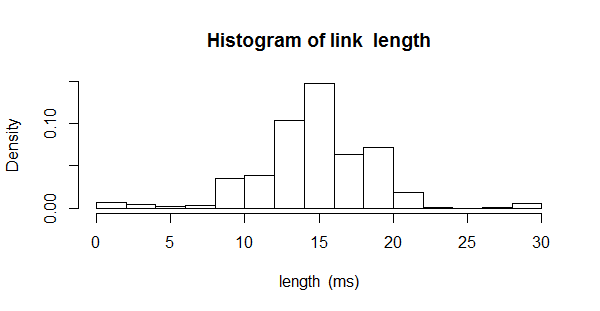
\includegraphics[width=0.95\textwidth, keepaspectratio]{figures/link-length-hist.png}
	\caption{Az útvonalak HOP számának eloszlása}
	\label{fig:link-len}
\end{figure}

Ellenőrzésként a mérésben résztvevő útvonalak késleltetése 93,3 milliszekundum átlagosan, a közbülső linkek száma pedig 15,3 átlagosan, ami igazolja a kimutatást. A linkek számáról részletesebb kimutatást a \ref{fig:link-len} ábra ad, amely a PlanetLab gépei közötti útvonalak HOP számának eloszlását mutatja.

A mérés legfőbb értékét az adja, hogy ezek a mérések nem egy hálózati pontból lettek indítva, hanem közel 200 csomópontból teljes hálót alkotva lettek elindítva a mérések. Ez olyan elemzésekre ad lehetőséget, mint az ú.n Hot-Potato jelenség megfigyelésére, amelyet korábbi kutatások is kimutatták\cite{hot-potato}.

\subsubsection*{A Hot Potato jelenség}

\begin{figure}[!ht]
	\centering
	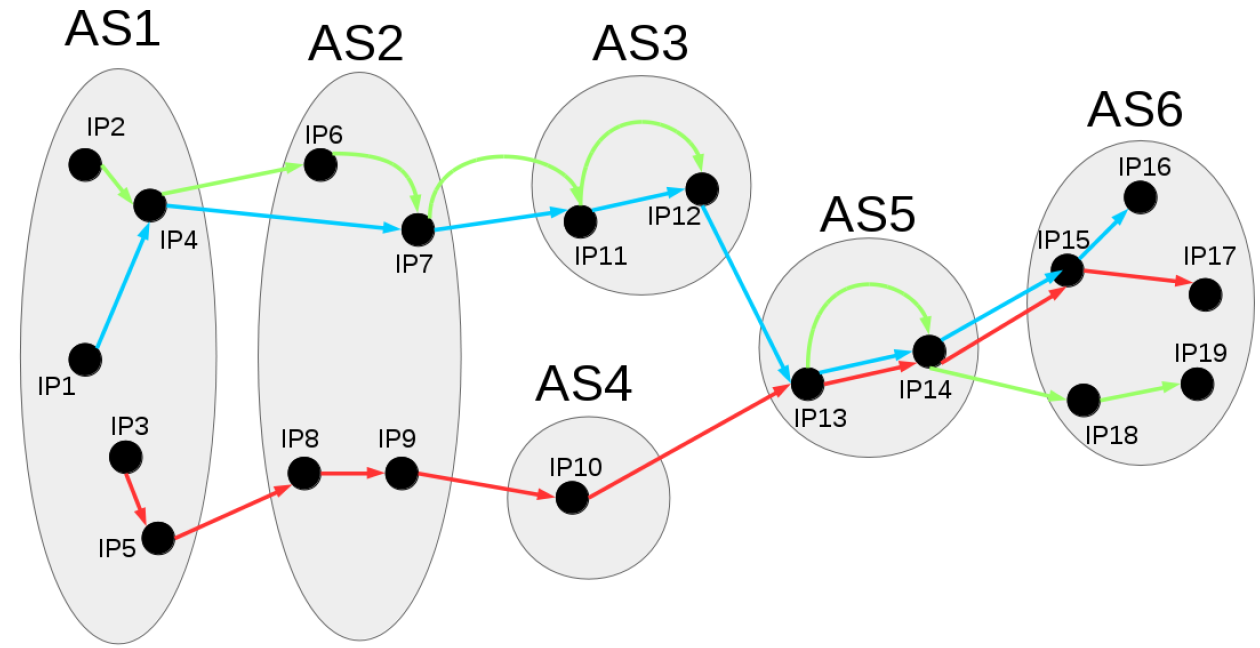
\includegraphics[width=0.7\textwidth, keepaspectratio]{figures/hot-potato.PNG}
	\caption{Csomagtovábbítási stratégia}
	\label{fig:hot-potato}
\end{figure}

\pagebreak

A \ref{fig:hot-potato} ábrán az látható, ahogy az AS1 ISP azonnal kivezeti a hálózatából a kék és piros küldendő adatcsomagot, hiába lettek azonos cél AS-hez címezve. A csomag továbbítása lefoglalná a saját erőforrásait. Ha más AS felé továbbítja, úgy mások erőforrásait használja. A szerződések ugyanis nem drágítják meg a csomagok továbbításának az árát, ha az távolabbra küldődik.

\begin{figure}[!ht]
	\centering
	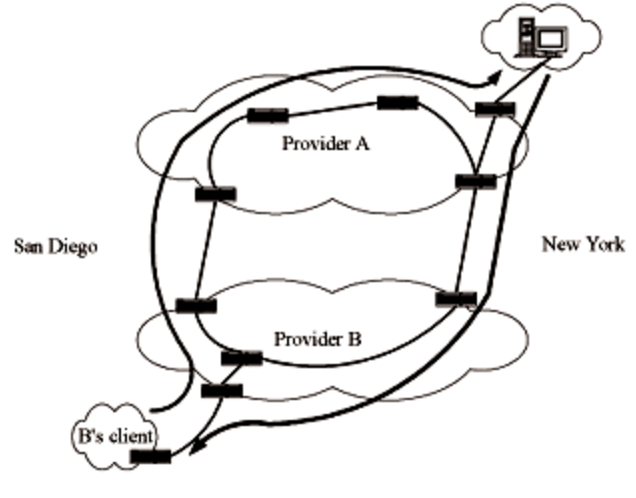
\includegraphics[width=0.4\textwidth, keepaspectratio]{figures/asymetric.PNG}
	\caption{Asszimetrikus útvonalválasztás a Hot-Potato jelenség miatt\protect\footnotemark}
	\label{fig:hot-potato}
\end{figure}

\footnotetext{Az ábra a \cite{hot-potato} forrásból lett átvéve}

A mérésekből úgy mutatható ki ez a stratégia, hogy azonos csomópont-pár esetén az egymás felé küldött csomagok nem feltétlen azonos útvonalon haladnak. Ugyanis a küldő ISP más útvonalat választ a hálózatából kifele küldött csomag számára, mint a fogadáskor.

\subsection*{PlanetLab gépek állapota}
A PlanetLab gépek eléréséről (az operációs rendszeréről) és hiba esetén a hibaüzenetek aggregált statisztikája. A következő adatokat tartalmazza:

\begin{itemize}
\item \textbf{erroneous:} Sikertelen csatlakozások száma (online gépek esetén)
\item \textbf{succeed:} Gépek száma, amelyeken sikeres volt a távoli parancsfuttatás (cat /etc/issue)
\item \textbf{online:} A ping parancssal elérhető gépek száma
\item \textbf{offline:} A ping parancssal nem elérhető gépek száma
\item \textbf{outputs:} Az összes különböző kimenet felsorolása a hozzá tartozó előfordulások számával.
\item \textbf{error\_types:} Az összes különböző hibatípus felsorolása a hozzá tartozó előfordulások számával
\item \textbf{ts:} A mérés időpontja
\end{itemize}

\begin{figure}[!ht]
	\centering
	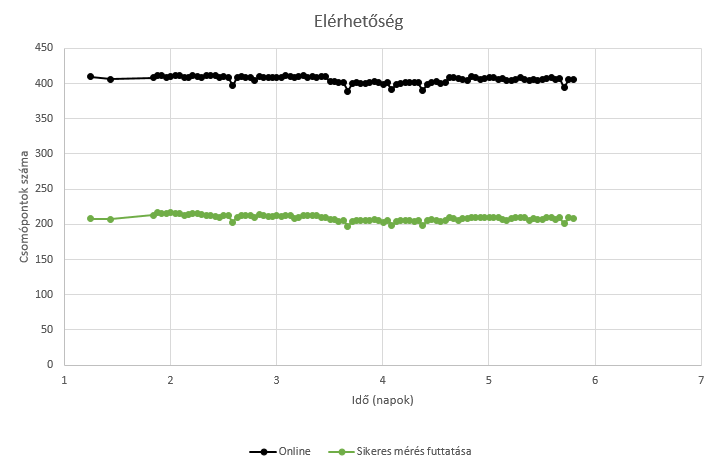
\includegraphics[width=0.9\textwidth, keepaspectratio]{figures/availability.PNG}
	\caption{A PlanetLab hálózat gépeinek elérhetősége egy hetes mintavételen}
	\label{fig:availability}
\end{figure}

Ez az adat kollekció a legfontosabb forrása a mérési rendszer rendelkezésre állásának és a hozzá szükséges PlanetLab hálózat elérhetőségének monitorozásának. A \ref{fig:availability} ábrán látható az online és a succeed adatsorok egy hetes mintavétele. Jól látható, hogy a PlanetLab hálózatának elérhetőségében van egy kevés fluktuáció, maximum 10 gép körüli szórással azonban összességében stabilan elérhetőek.



\subsection*{AS gráf él információi}
A korábban részletesen bemutatott AS gráf ezen kollekció adataiból lett felépítve:

\begin{itemize}
\item \textbf{asn:} A autonóm rendszer azonosító száma
\item \textbf{core\_ips:} Az autonóm rendszeren belül észlelt ip címek
\item \textbf{gateways\_to\_as:} Az autonóm rendszerből másikba vezető kapcsolatok listája. A másik AS-hez irányuló ip cím párok (egyik AS kimeneti címe, másik AS bemeneti címe) listáit is tartalmazza.
\end{itemize}

Ezen adatsor bemutatása nagy részben a következő szekcióban történik majd, mivel az elkészült gráfok adatforrása ez az adat kollekció. Az eredményezett gráf megjelenítéshez viszont nem kapcsolódó kimutatás látható a \ref{fig:as-route-len} ábrán, amely a feltérképezett Autonóm Rendszerek közötti útvonalak hossz eloszlását ábrázolja.

\begin{figure}[h!]
	\centering
	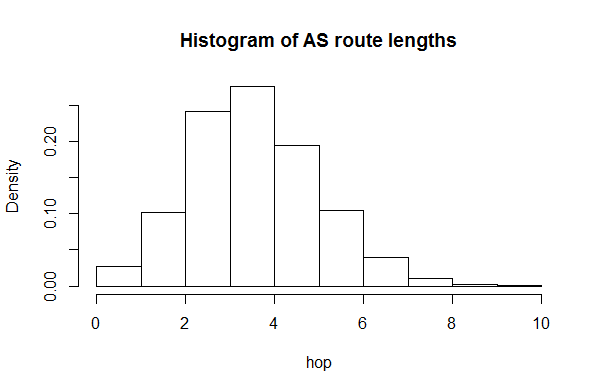
\includegraphics[width=0.9\textwidth, keepaspectratio]{figures/as-hop-hist.png}
	\caption{Az AS gráf csomópontjai között lévő útvonalak hosszának eloszlása}
	\label{fig:as-route-len}
\end{figure}

Az IP linkek és az AS linkek természetes hasonlósága okán a korábbi \ref{fig:link-len} ábrához hasonlít. Az útvonalak hosszának függetlensége miatt a centrális határeloszlás értelmében minél nagyobb a mérés mintavétele, annál jobban hasonlítanak az említett függvények a Normális eloszlásra. Az AS gráf az egy \glqq klaszterhez \grqq tartozó IP csomópontok egybeolvasztása révén jön létre. A kapott hálózat pedig legtöbb tulajdonságát így örökli az eredeti gráfból.


\section{Gráfok ábrázolása}

\begin{figure}[!h]
	\centering
	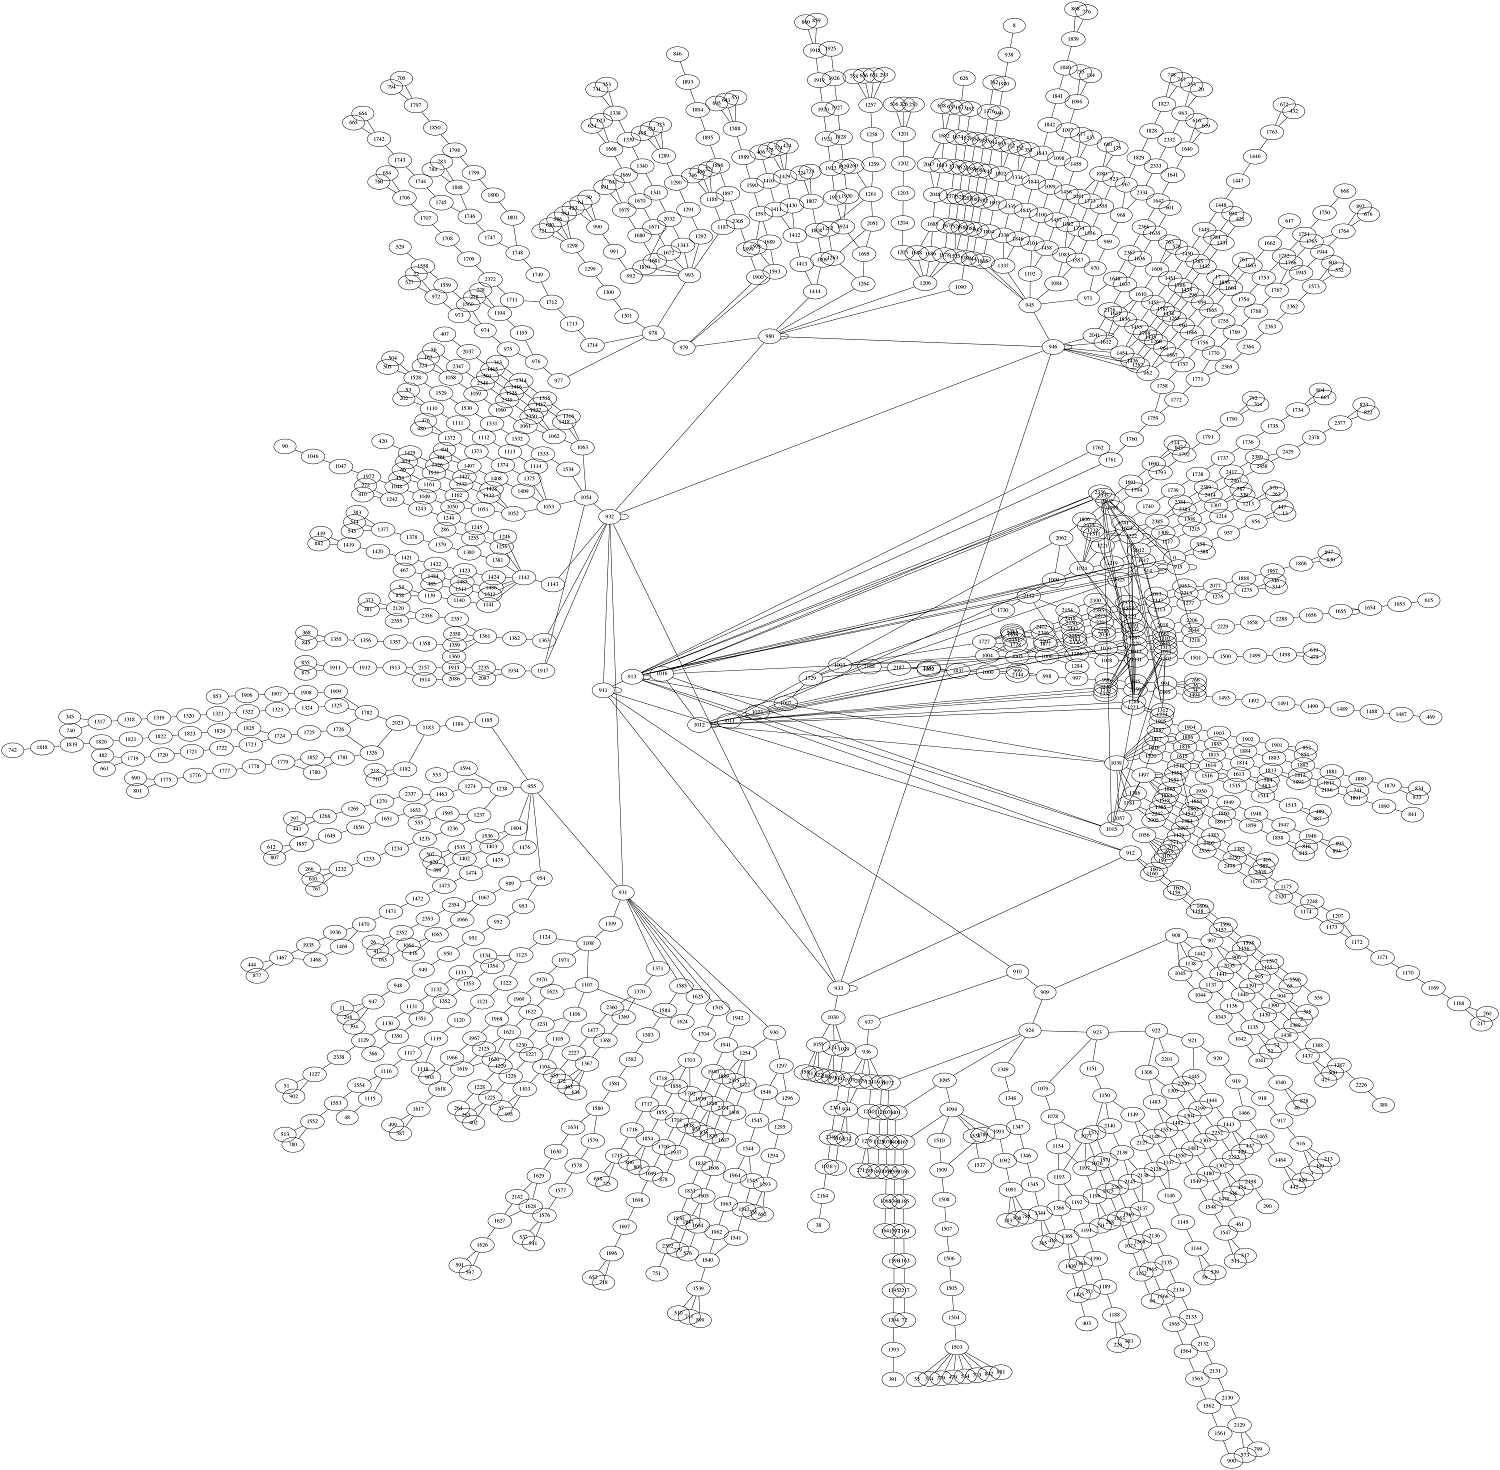
\includegraphics[width=1\textwidth, keepaspectratio]{figures/graph.png}
	\caption{Egy napi mérés gráfja egy egyetemi cím felé vezető útvonalak IP csomópontjaiból\label{fig:graph}}
\end{figure}

A mérési eredményekből készült gráfok tulajdonságainak intuitív leolvasásához ábrázolások készültek. Mivel egy mérés során több mint 1700 csomópontból álló gráfot kell ábrázolni, ezért ennek kivitelesése kihívást jelent. A \ref{fig:graph} ábrán látható az első sikeres gráf ábrázolás, amelyen már kivehető a gráf szerkezete.
Az ábrán jól láthatóak a középponttól távolodó hosszú fürtök, melyek egy cél IP címhez vezető többnyire független útvonalakat reprezentálja.

\pagebreak


\begin{figure}[!h]
	\centering
	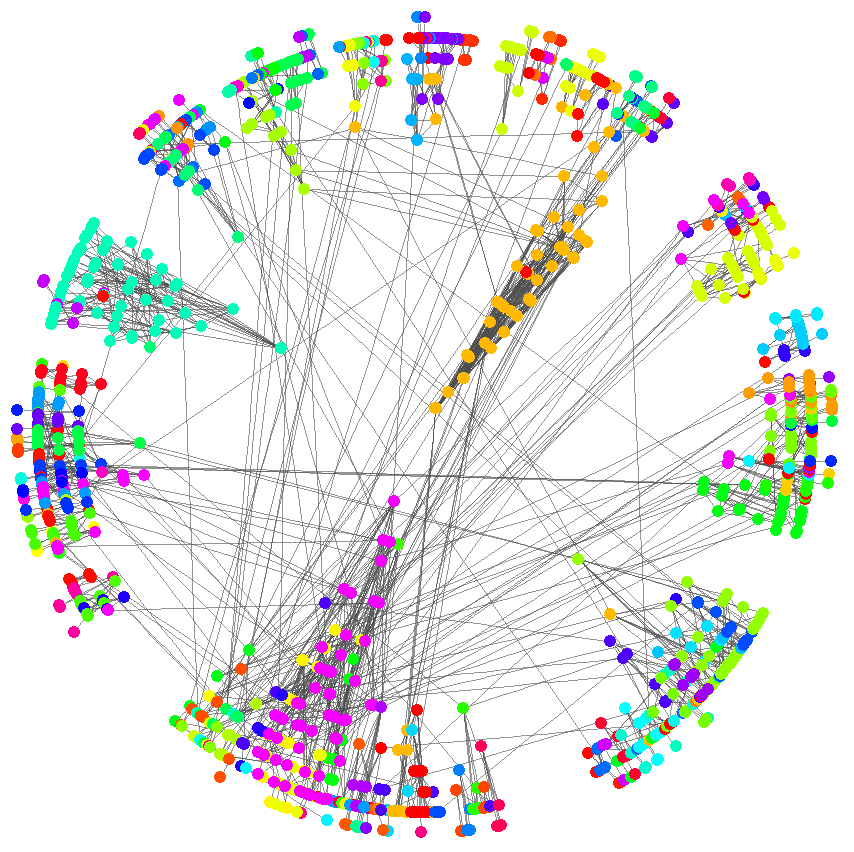
\includegraphics[width=1\textwidth, keepaspectratio]{figures/as-graph2.png}
	\caption{Az IP gráf továbbfejlesztett ábrázolása\label{fig:ip-graph}}
\end{figure}

Az ábrázolás további fejlesztését követően a \ref{fig:ip-graph} ábrán látható kép készült el. Ezen az egyes IP csomópontok sugárirányban a fokszámuk alapján vannak elhelyezve, minél nagyobb fokszámmal rendelkeznek, annál közelebb vannak az origóhoz. Ezen felül klaszterezést követően lettek csoportonként szétszórva a kör peremén. A színezés az egy AS-hez tartozó IP csomópontokat jelöli. A legtöbb esetben a klaszterezés vissza is adta a csomópontok Autonóm Rendszerekhez való rendelését. A kör közepén a korábban említett alacsonyabb Tier szinthez tartozó Autonóm Rendszerek csomópontjai tartoznak.

\pagebreak

A csomópontok koordinátáinak számításához használt funkció a következő volt, amely az R programozási nyelven lett írva:

\begin{lstlisting}[language=R]
my_layout <- function(net){
  # Alap informaciok kinyerese a halozatbol
  nodes = V(net)
  deg = degree(net)
  max_deg = max(deg)
  clust = cluster_louvain(net)
  memb = membership(clust)
  
  # klaszterek szogtartomanyokra osztasa
  group_start = get_group_start_indexes(memb, nodes)
  
  for(n in nodes){
    group = memb[n]
    # origotol valo tavolsag szamitasa
    radius = (max_deg - deg[n] + 1)/(max_deg + 1)
    # klaszterek alapjan valo csoportositas
    angle = step * ( group_start[group] + group_index[group] )
    group_index[group]  = group_index[group] + 1
    
    coord[n, 1] = radius * cos(angle)
    coord[n, 2] = radius * sin(angle)
  }
  
  return(coord)
}
\end{lstlisting}


\pagebreak

\begin{figure}[h!]
	\centering
	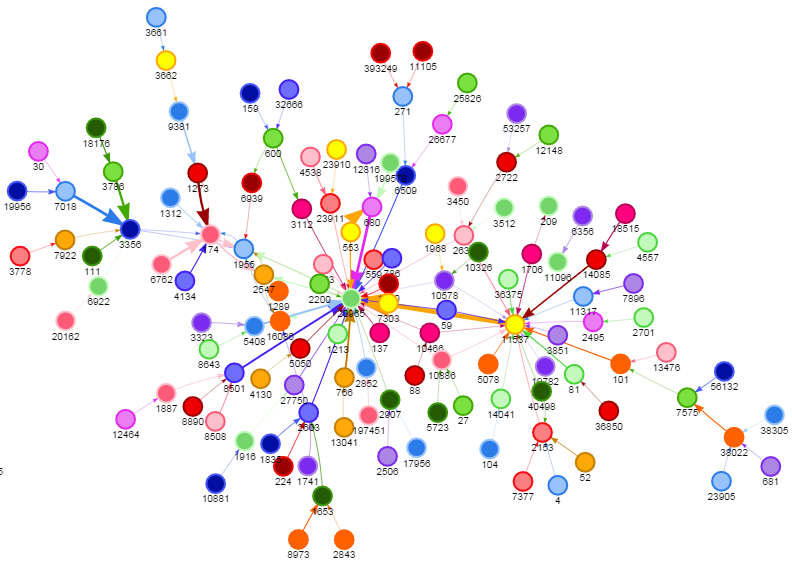
\includegraphics[width=0.95\textwidth, keepaspectratio]{figures/as-graph.png}
	\caption{A PlanetLab gépeitől az egyetem felé küldött csomagok által bejárt AS gráf}
	\label{fig:as-graph}
\end{figure}


Az AS szám információ felhasználásával a \ref{fig:as-graph} ábrán látható gráf lett elkészítve. Az ábra adatforrása pár nap folyamatos traceroute mérések eredménye. A PlanetLab csatlakozott gépeiről a BME egyik gépe felé címzett útvonalak lettek aggregálva. A nyilak vastagsága az alapján növekszik, hány különböző IP cím pár közti össze a két AS csomópontot. Ha minden átmenő csomag azonos IP címeken halad keresztül akkor az vékony lesz, míg ha két AS között haladó csomagok több különböző IP cím párokon keresztül utaznak az vastagabban van ábrázolva.

A \ref{fig:as-graph} ábráról leolvasható, mely Autonóm Rendszerek földrajzilag kiterjedtek. Ha ugyanis több különböző IP útvonal köt össze két AS-t akkor azok valószínűleg területileg is több ponton vannak összeköttetésben.

A \ref{fig:as-graph} ábrán az összes útvonal a BME AS2547-es csomópontjába irányul, amely a valóságban kizárólag a AS1955-ös HBONE-AS HUNGARNET-tel van összeköttetésben. Egyes hibás traceroute mérések azonban torzítják ezt. A legnagyobb fokszámú csomópont az AS20965 , amely az AS1955 legfontosabb szomszédja, az elvi 17-ből\footnote{Forrás: Európai Regionális Internetes Nyilvántartó Hivatal honlapja: \href{https://stat.ripe.net/widget/asn-neighbours\#w.resource=1955}{stat.ripe.net}}.

%\begin{figure}[h!]
%	\centering
%	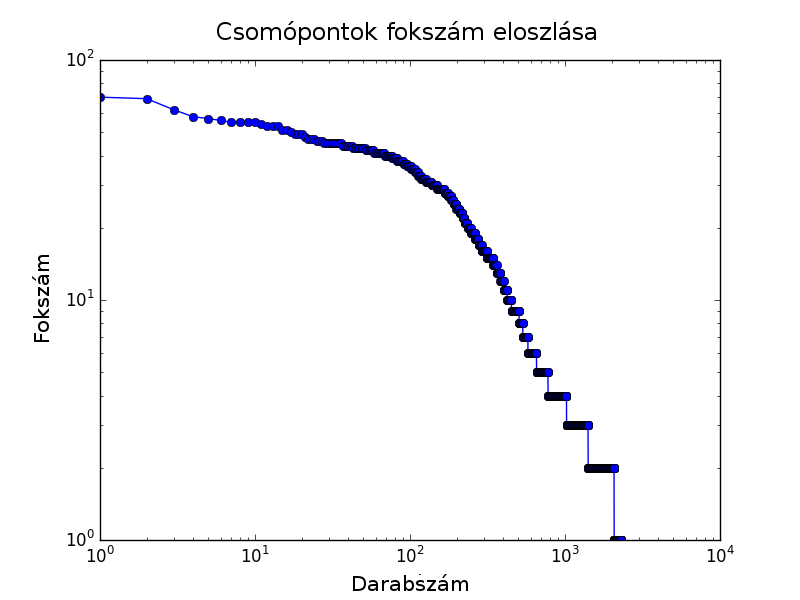
\includegraphics[width=0.95\textwidth, keepaspectratio]{figures/degree.png}
%	\caption{Az IP gráf csomópontjainak fokszáma előfordulási sűrűségük függvényében}
%	\label{fig:ip-degree}
%\end{figure}


\begin{figure}[h!]
	\centering
	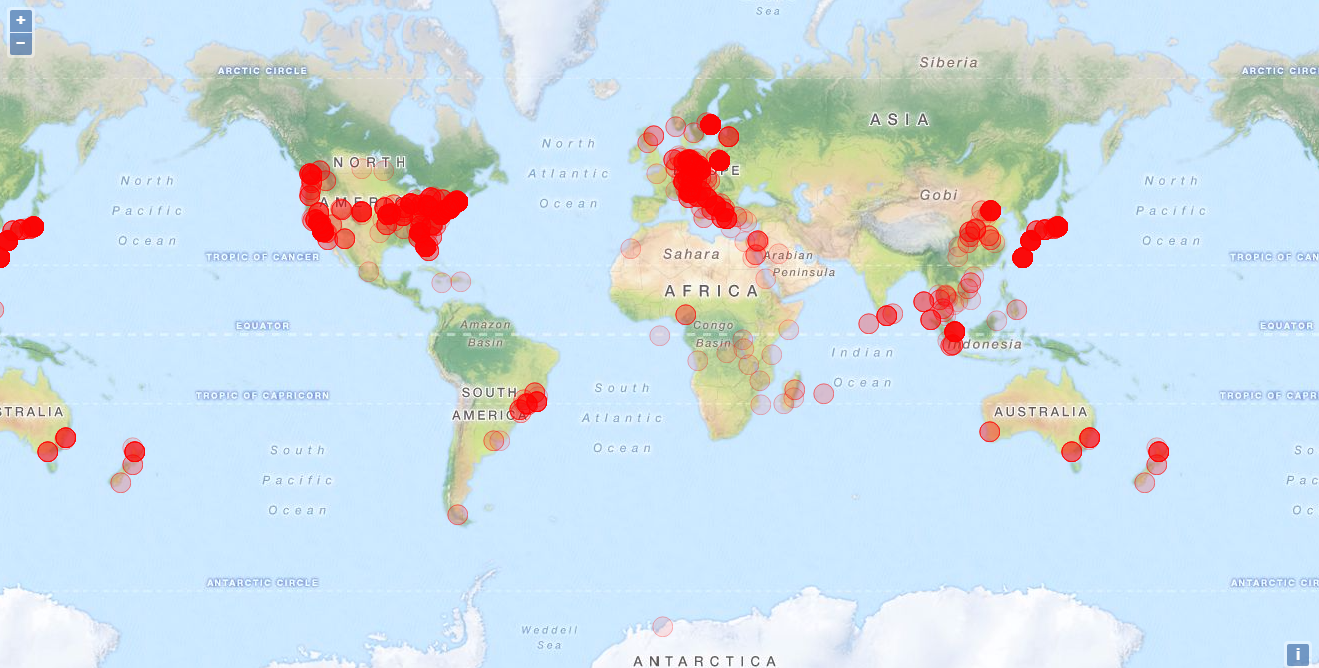
\includegraphics[width=0.9\textwidth, keepaspectratio]{figures/ip_map.png}
	\caption{A mérésben résztvevő IP címek geolokációs pozíciójai}
	\label{fig:ip-map}
\end{figure}

Az IP csomópontok geolokációs adatokkal való felgazdagítását követően új ábrázolási mód vált elérhetővé az Internet szerkezetének a megfigyeléséhez. Ennek eredménye a \ref{fig:ip-map} ábrán látható. A mérések reprezentativitását bizonyítja az Internetes penetrációval rendelkező területek nagy részén látható mérésben résztvevő csomópontok sokasága.

\pagebreak

\section{Middlebox felderítés}
A tanszéken végzett Internetes kutatásokhoz hozzáadott értéket jelentett a mérési rendszer. A kutatás középpontjában napjaink egyik Internetes trendje az úgynevezett Middlebox-ok voltak. Ez egy általános fogalom minden olyan hálózati eszközre vonatkozóan, amely beavatkozik és manipulálja a rajta átmenő forgalmat. Ilyen lehet a hagyományos tűzfal vagy terheléselosztó, de manapság újabb és újabb célra használják fel, néha beavatkozva a végpontok közötti kapcsolatba. Ez az Internet alapjait jelentő protokollok működésére akár nem kívánt hatással is lehet, ezért fontos kutatási téma napjainkban.

A kutatáshoz való hozzájárulása a mérési rendszernek az interneten küldött csomagok TTL mezőjének a manipulációját vizsgálta. Egy célgépen a tcpdump nevű alkalmazást volt elindítva olyan beállításokkal, hogy csak a mérésben résztvevő csomagokat vizsgálja. A PlanetLab hálózat elérhető gépein pedig speciálisan elkészített csomagok voltak küldve a célgép felé a maximális 250-es TTL mezővel. A vizsgálat a Middlebox-ok TTL manipulációját figyelte a különböző csomagtípusokra vonatkozóan.

Három csomagtípus manipulációja volt vizsgálva:

\begin{itemize}
\item \textbf{ICMP Ping request} Hagyományos ping üzenet kérési csomagja
\item \textbf{TCP SYN port:22} TCP kapcsolatfelépítési csomag a 22-es portra, amely az ssh kapcsolatok fogadására szolgál
\item \textbf{TCP SYN port:80} TCP kapcsolatfelépítési csomag a 80-as portra, amely a http kapcsolatok fogadására szolgál
\end{itemize}

A felhasznált parancsok a következők voltak:

\begin{lstlisting}[language=bash]
  # Celgepen futtatott parancs ICMP csomagok fogadasara
  sudo tcpdump -vnn -i eth0 icmp[icmptype] == 8 and dst host $ip
  # PlanetLab gepekrol kuldott ICMP csomagok parancsa
  ping -c 1 -t 250 $ip
  
  # A celgepen futtatott parancs TCP SYN csomagok fogadasara
  sudo tcpdump -vnn -i eth0 dst host $ip and "tcp[tcpflags] & (tcp-syn) != 0"
  # A PlanetLab gepeirol kuldott TCP csomagok parancsa
  nmap -v --ttl 250 --max-retries 1 -PS -p 80 $ip
  nmap -v --ttl 250 --max-retries 1 -PS -p 22 $ip
\end{lstlisting}


A mérés egy korábbi tanulmányt\cite{middlebox} vett alapul a felderítéshez. Az Internetes útvonalakon található, ttl mezőt manipuláló Middlebox-ok jelenlétét kimutatta a mérés. A mérés 75 szerverről küldött csomagok alapján lett elkészítve, mindegyik csomagtípusból egyet küldve a célgép felé, kivéve a 80-as portra küldöttek, amelyekből 3 csomag lett küldve gépenként.


\begin{figure}[!ht]
	\centering
	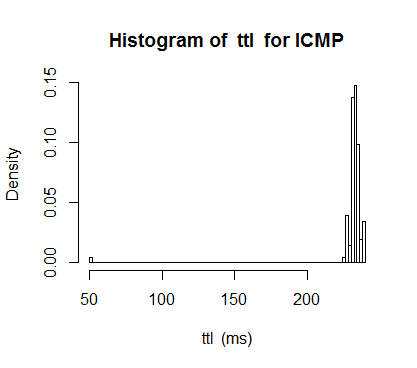
\includegraphics[width=0.3\textwidth, keepaspectratio]{figures/hist-ttl-icmp.png}
	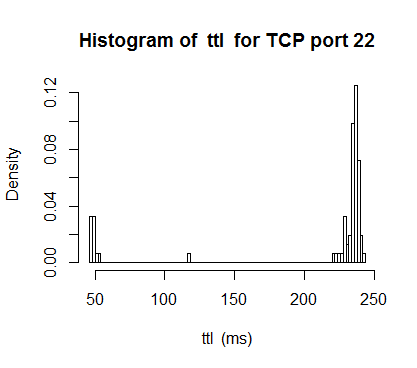
\includegraphics[width=0.3\textwidth, keepaspectratio]{figures/ttl-hist-22.png}
	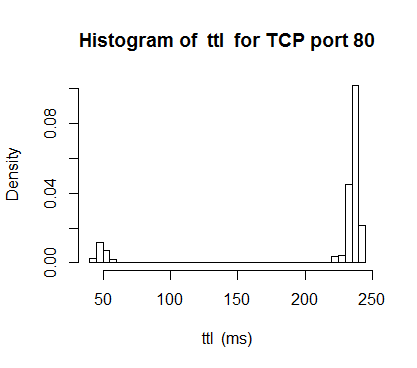
\includegraphics[width=0.3\textwidth, keepaspectratio]{figures/ttl-hist-port80.png}
	\caption{A fogadott csomagok TTL értékeinek előfordulási sűrűsége}
	\label{fig:ttl-hist}
\end{figure}

A \ref{fig:ttl-hist} ábrán látható, hogy az eredetileg 250-es TTL mezővel küldött csomagok egy része fogadáskor már egy közbülső elem által manipulálva lett. A manipuláció abból következtethető, hogy az útvonalak hosszúsága normális eloszlást követ, ahogy a \ref{fig:hop-hist} ábrán látható, valamint a TTL csökkenésnek függetlennek kellene lennie a csomag típusától.

\begin{figure}[!ht]
	\centering
	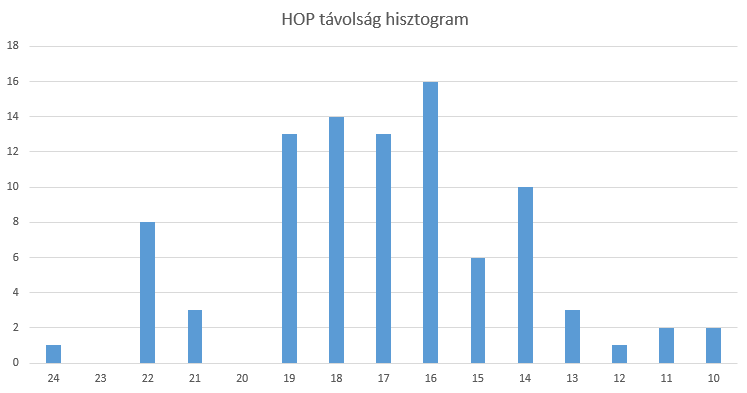
\includegraphics[width=0.5\textwidth, keepaspectratio]{figures/hop-hist.png}
	\caption{Az eredeti HOP távolsága a mért útvonalaknak}
	\label{fig:hop-hist}
\end{figure}

Az ICMP csomagok ábráján egyetlen csomag érkezett vélhetően módosított TTL mezővel, későbbi ellenőrzéskor azonban kiderült, egy nem a mérésben résztvevő gép küldte. A méréshez használt csomagszűrő minden Ping requestet átengedett, azonban a mérés ideje alatt a colorado-i egyetem egyik szervere is küldött ilyen csomagot, valószínűleg más Internetes mérés részeként. Ilyen módon kimondhatjuk, hogy az ICMP csomagok TTL mezője nem megy keresztül módosításon. Ezzel szemben a TCP csomagok, amelyeket vizsgáltunk az esetek több mint 10\%-ában módosításon estek keresztül. A 80-as portra küldöttek 11\%-a, míg a 22-es portra küldöttek 15\%-a. Itt megjegyzendő, hogy nem következetes az útvonalakon közbeiktatott manipuláció. Egyes útvonalakon csak a 22-es portra küldött csomagok lettek változtatva, másokon csak a 80-as portra küldöttek és természetesen legtöbb esetben mindkettő. Ezen felül a 80-as portra küldött 3 csomagból, manipuláció esetén a legtöbb esetben egyszerre voltak csökkentett TTL mezőjűek és érintetlenek is.

A vélhető ok, amiért az ICMP csomagokak érintetlenül hagyják a Middlebox-ok, az az ICMP csomagok hálózatdiagnosztikai természetéből adódik. Ezeket valószínűleg a hálózat helyes működésének ellenőrzéséhez is használják az operátorok. A hálózat egészséges működésének érdekében ezért támogatniuk kell az ICMP csomagok továbbításának a protokolloknak megfelelő módját.

Ez a mérés jól mutatja be a mérési rendszerben rejlő potenciált. A PlanetLab hálózatnak köszönhetően, az Internetre reprezentatív eredmények jöhetnek létre a gyorsan összeállítható mérési forgatókönyveknek hála.
%Mérési eredmények (7-10 oldal): kinyert mérések tartalma(delay, jitter, link, AS info, Geolocation), mérések mennyisége, mérések minősége

%
\section{Adatok feldolgozása}
(5 oldal): Hibák kiszűrése, gráf reprezentálás, statisztikák
\citep{traceParse}
%Adatok feldolgozása (5 oldal): Hibák kiszűrése, gráf reprezentálás, statisztikák


%------------------------------------------------
% Együttműködések (6 oldal): Hogyan csatlakoztak be, mit értek el, mivel lett több az egész, együttműködések menete.
\chapter{Kiegészítő modulok}
%(6 oldal): Hogyan csatlakoztak be, mit értek el, mivel lett több az egész, együttműködések menete.

% Mit adott hozzá az én témámhoz?
% Az én témámnak mely részeire tudta építeni a saját munkáját?

A mérési rendszer fejlesztése 2015 tavaszi félévében kezdődött önálló laboratóriumi munkaként. Az első működő verziót követően további témakiírások készültek hozzá kapcsolódóan. Ezek közreműködési lehetőséget biztosítottak a hallgatóknak, hogy saját munkájuk során a meglévő mérési rendszert vagy annak eredményeit felhasználják és kiegészítsék azt. A következőkben ezen munkák kerülnek bemutatásra. Az egyes leírások fontos eleme a mérési rendszerhez való hozzáadott értékek és a rendszer felhasznált szolgáltatásainak kiemelése.

Ezen együttműködéseknél rendkívül fontos volt az ismeret átadás, és a munkák koordinálása. A konzulensemmel, Dr Heszberger Zalánnal, végig gondot fordítottunk arra hogy minden szükséges tudást átadjunk a munkákhoz, és felügyeljük azok végrehajtását. Minden esetben elégedettek voltunk a közös munka gyümölcsével, és sokszor kellemesen meglepett milyen távolra vezettek az általunk elindított témák.

Az egyes fejezetcímek az elkészült dolgozatok címének felelnek meg.


%%%%%%%%%%%%%%%%%%%%%%%%%%%%%%%%%%%%%%%%%%%%%%%%%%%%%%%%%%%
\section{Forgalmi mérési környezet}
%Haja Dávid munkájának rövid bemutatása (2 oldal)


%%%%%%%%%%%%%%%%%%%%%%%%%%%%%%%%%%%%%%%%%%%%%%%%%%%%%%%%%%%
Haja Dávid alapszakos hallgató a szakdolgozataként választotta az általunk kiírt témát 2015 őszi félévében. Munkája során megismerte az Elméleti Áttekintés fejezet tudásanyagát, valamint a mérőrendszer felépítését. Fő tevékenységei a PlanetLab hálózat komolyabb megismerése volt, valamint a mérési rendszer kiegészítése sávszélesség kapacitás méréssel.

\subsection*{PlanetLab rendszerének megismerése}
A mérések végrehajtása során a PlanetLab hálózat gépeinek elérésével gondjaink akadtak. A tanszéken üzemelő szerverek nem megfelelően voltak felkonfigurálva, nem üzemeltek rendeltetésszerűen. A kölcsönösség elve alapján így nem fértünk hozzá a PlanetLab hálózatának szervereihez.
Haja Dávid közreműködésével az említett szerverek helyre lettek állítva. Ezen munkája során mély ismeretekre tett szert a PalnetLab szervezet működésével és a szerverek felépítésével kapcsolatban.

\subsection*{D-ITG sávszélesség mérés}
A mérési rendszer eredetileg csak iperf sávszélesség mérésekkel rendelkezett, mivel ez a szoftver a legtöbb linux alapú rendszereken, így a PlanetLab gépein is, előre telepítve volt. A mérések színvonalának érdekében azonban Haja Dávid feladata volt felmérni mely további sávszélességmérő rendszerek nyújthatnak megbízható és részletes mérési adatokat. Kutatásai során választása a D-ITG-re (Distributed Internet Traffic Generator) esett. Ez a mérőszoftver bír az elvárható alapképességekkel, mint a kinyerhető adatok széles választéka, protokoll támogatások, párhuzamos folyamok kezelése, valamint sztochasztikus adatküldő profilok is beállíthatóak. A program azonban nem elérhető a publikus csomagkezelő rendszerekből, ahonnan egyszerűen telepíthetőek lennének. Emiatt munkájának nagy része volt a szoftver becsomagolása a PlantLab gépeinek megfelelő RPM formátumba. 
Az így elkészült telepítőcsomagok automatizált telepítését az Ansible szoftverrel oldotta meg.

Munkájának gyümölcseként új mérési lehetőségekkel bővült az eredeti rendszer. Az új mérési típus nem jöhettek volna létre a mérési rendszer rugalmassága által, a rendszer forráskódjában egyetlen osztály létrehozására volt szükség az új funkció implementálásához. Az új képességeket jól mutatja be az alábbi mérési eredmény, amely két különböző, ám hálózati szempontból közel lévő cél felé indít sávszélesség méréseket. 

\begin{figure}[!ht]
	\centering
	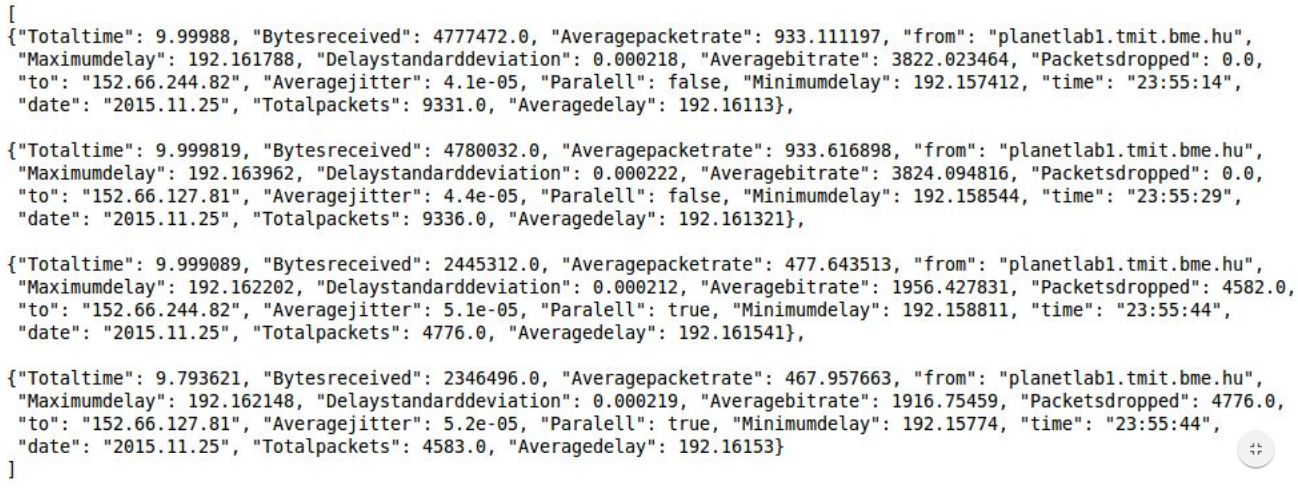
\includegraphics[width=0.95\textwidth, keepaspectratio]{figures/d-itg-measure.PNG}
	\caption{Sávszélesség mérési forgatókönyv eredménye}
	\label{fig:d-itg-measure}
\end{figure}

\newpage

A \ref{fig:d-itg-measure} ábrán látható mind a négy részeredmény ugyanahhoz a mérési forgatókönyvhöz tartozik. Alább részletezem az egyes részmérések tartalmát:

\begin{itemize}
 \setlength{\parskip}{0pt}
 \setlength{\itemsep}{0pt plus 1pt}
 
\item 10 másodperces mérés az első cél felé
\item 10 másodperces mérés a második cél felé
\item 10 másodperces mérés parallel a két cél felé, az első cél folyamának eredményeit prezentálva
\item 10 másodperces mérés parallel a két cél felé, a második cél folyamának eredményeit prezentálva
\end{itemize}


%%%%%%%%%%%%%%%%%%%%%%%%%%%%%%%%%%%%%%%%%%%%%%%%%%%%%%%%%%%
\section{AS útvonalváltozás elemzések}
%Kocsmár Bence munkájának rövid bemutatása (2 oldal)


%%%%%%%%%%%%%%%%%%%%%%%%%%%%%%%%%%%%%%%%%%%%%%%%%%%%%%%%%%%
Kocsmár Bence alapszakos hallgató szakdolgozataként választotta a konzulensemmel együtt kiírt témánkat a 2016-os év tavaszi félévében. Közreműködése mutatja a legjobban a mérési rendszerben lévő potenciált, ez volt az első olyan munka amely nem a mérések végzéséhez járult hozzá, hanem a kinyert adatokat dolgozta fel. Munkája során a traceroute alapú mérésekből kinyert ip útvonalak adatait dolgozta fel. A BGP útvonalhirdetések alapján felmért AS útvonalakkal szemben ilyen módon az útvonalakon való csomagkésleltetési idők is rendelkezésre álltak, ami többlet információkkal szolgált.

A mérési rendszer által kinyert adatok több adatfeldolgozási folyamaton mentek keresztül, melynek során külön adatstruktúrában lettek tárolva az autonóm rendszerek belső csomagtovábbítási tulajdonságai és az AS szintű csomagtovábbítási információk. Ezt a feldolgozási lépést követően az azonos forrás-cél útvonalakhoz tartozó adatok aggregálásra kerülte, hogy később historikus elemzést lehessen rajtuk végezni.

\subsection{Új AS kapcsolatok felderítése}

\begin{figure}[!ht]
	\centering
	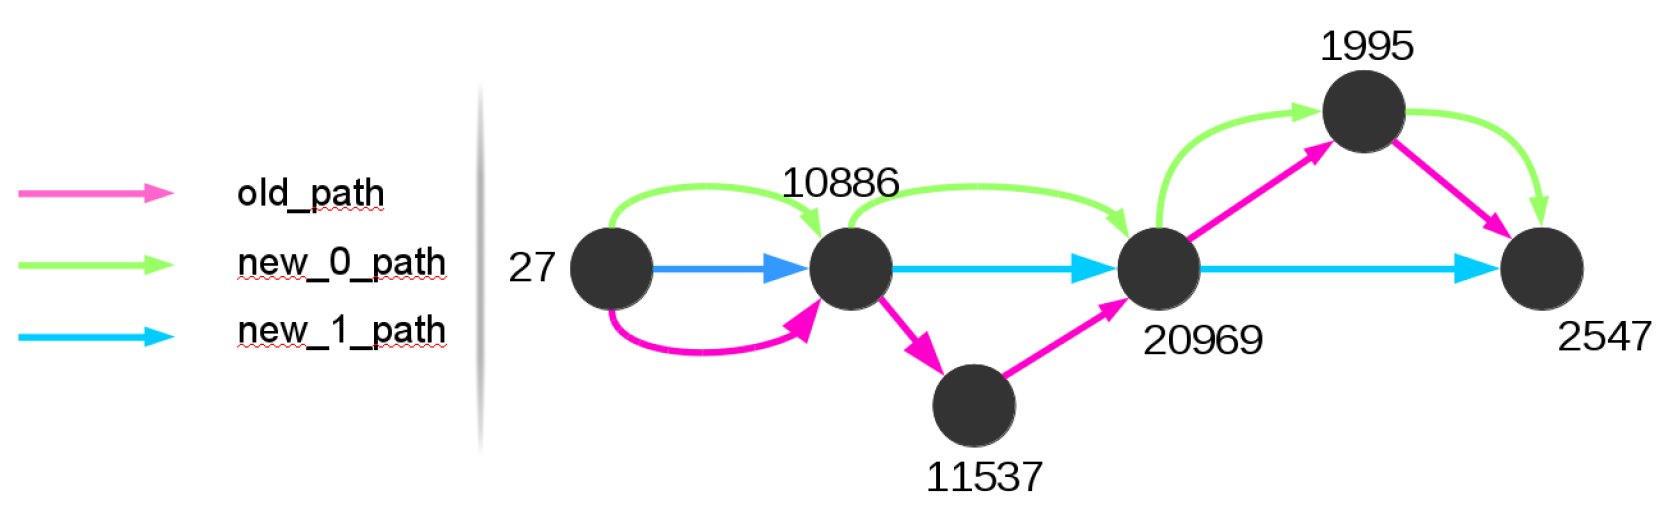
\includegraphics[width=0.70\textwidth, keepaspectratio]{figures/as-path-change-graph.PNG}
	\caption{AS-es között felderített útvonal kapcsolatok}
	\label{fig:as-path-change-graph}
\end{figure}

A kinyert AS útvonalak adatai útvonalváltozások észlelésére lettek felhasználva. A \ref{fig:as-path-change-graph} ábrán egy ilyen útvonalváltozás van reprezentálva, ahol a mérések során három különböző útvonal lett detektálva ugyanazon ip forrás és cél esetén. A lila útvonal volt legelőször használatban, majd idővel két új jött létre. Az új útvonalak mind kevesebb AS-t érintettek, ami arra a következtetésre ad okot, hogy új AS összeköttetés jött létre. A legújabb, kék útvonal, szintén rövidebb a korábbi zöldnél. Az ilyen új AS partnerkapcsolatok létrejötte mutatja a szolgáltatók igyekezetét arra, hogy minél jobb minőségű, minél rövidebb csomagtovábbítási útvonalakat építsenek ki egymás között. 

\begin{figure}[!ht]
	\centering
	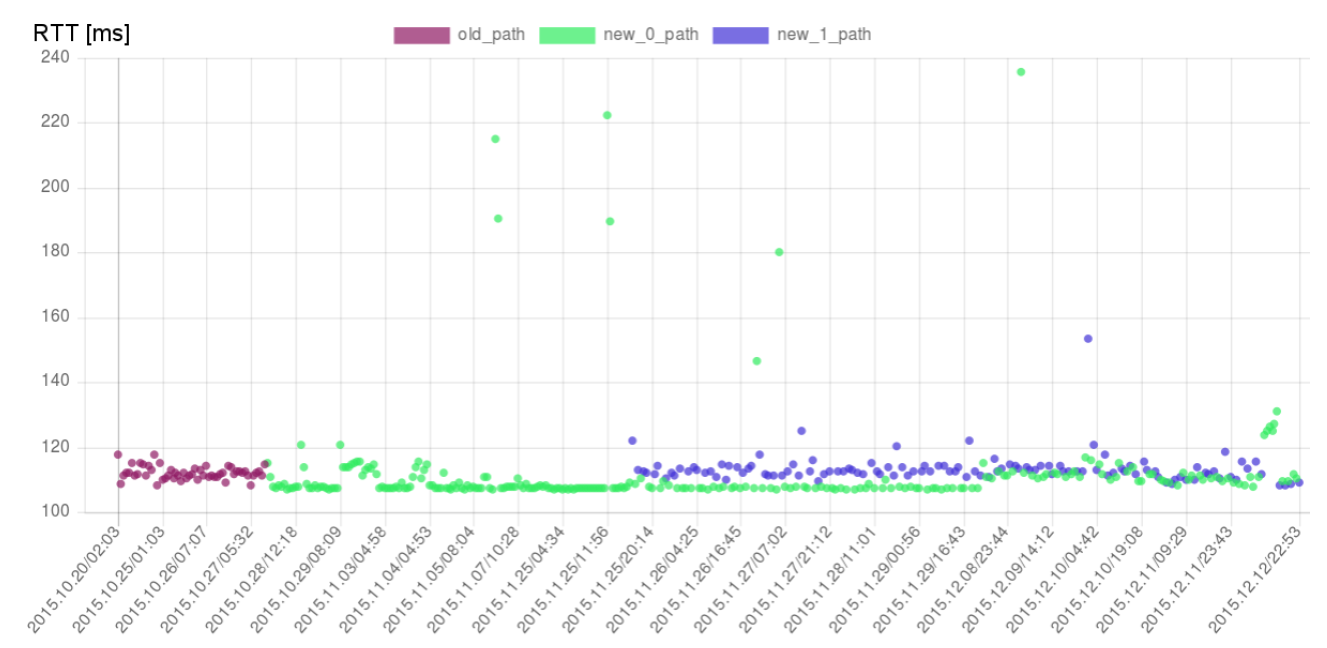
\includegraphics[width=0.95\textwidth, keepaspectratio]{figures/as-path-change-diagram.PNG}
	\caption{AS útvonalak használatának időbeli lefutása és késleltetéseik}
	\label{fig:as-path-change-diagram}
\end{figure}

A \ref{fig:as-path-change-graph} ábránál sokkal több információ olvasható le a \ref{fig:as-path-change-diagram} ábráról, amely nem csak az útvonalak időbeli feléledéseit mutatja, hanem a csomagkésleltetési tulajdonságokat. Erről leolvasható hogy az első útvonal gyakorlatilag megszűnt, ezzel szemben a két új útvonal felváltva vannak használva. Ennek oka lehet kapacitáselosztás vagy kísérleti üzem is. Ezt a sejtést megerősíti, hogy a RIPE szabadon elérhető adatbázisa\footnote{\url{https://apps.db.ripe.net/search/query.html}} alapján 2014 februárjáig nem volt összeköttetés az 10886-os s a 20965-ös AS között. A 20965-ös AS szám a GEANT szolgáltatóhoz tartozik, amely rendkívül nagy európai hálózattal és kapacitásokkal rendelkezik. A trend alapján a kisebb AS-ek igyekeznek közvetlen összeköttetést kiépíteni hozzá. A \ref{fig:as-path-change-diagram} ábráról mindezeken felül megállapítható, hogy a zöld útvonal rendkívül stabil 111 ms-os késleltetést garantált, amely kicsit gyorsabb a többinél, mindezt pedig kisebb variancia mellett.

\subsection{További útvonal információk}

A vizsgálatok fókuszában az AS útvonalváltozások álltak, azonban további tulajdonságok is kimutathatóvá váltak a mérési rendszer adatainak feldolgozásával. Erre egy említésre méltóbb példa az egyes autonóm rendszerek belső csomagtovábbítási eljárása. A \ref{fig:as-inside} ábrán a belső továbbítás során átlagosan érintett IP csomópontok száma látható az egyes AS-ek esetében.

\begin{figure}[!ht]
	\centering
	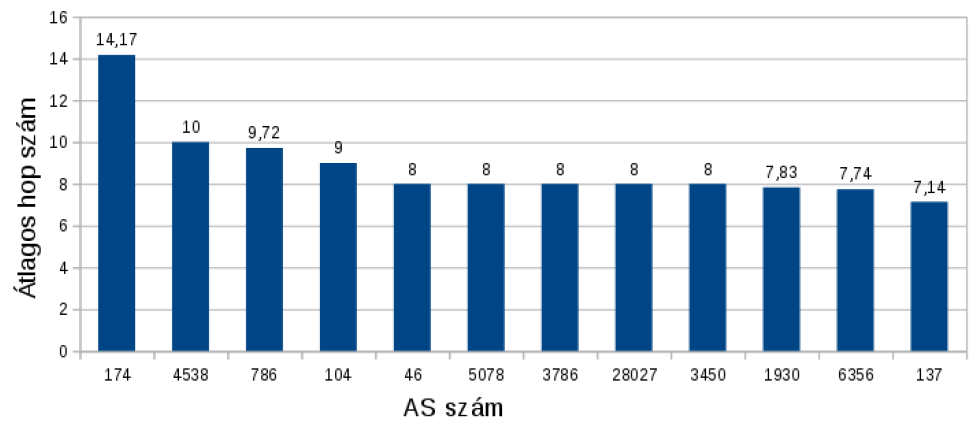
\includegraphics[width=0.9\textwidth, keepaspectratio]{figures/as-inside.PNG}
	\caption{Az autonóm rendszerek belső átlagos hop száma}
	\label{fig:as-inside}
\end{figure}

A mérések során leghosszabb belső hop számmal az amerikai Cogent tier 0-ás szolgáltató állt, átlagosan több mint 14 csomóponttal, amely a CAIDA által számított sorrend\footnote{\url{http://as-rank.caida.org/}} alapján a második legnagyobb AS. A második legtöbb hop számmal a 4538-as AS számú China Education and Research Network Center rendelkezett, amely a 1921-es a CAIDA rangsorában.


%%%%%%%%%%%%%%%%%%%%%%%%%%%%%%%%%%%%%%%%%%%%%%%%%%%%%%%%%%%
\section{Felhő alapú környezet}
%Patkó Ákos munkájának rövid bemutatása (1-2 oldal)


%%%%%%%%%%%%%%%%%%%%%%%%%%%%%%%%%%%%%%%%%%%%%%%%%%%%%%%%%%%
Patkó Ákos alapszakos hallgató önálló laboratóriumi témaként választotta a mérési rendszerhez tartozó kiírásunkat a 2016-os tavaszi félévben. Munkája során korábbi üzemeltetési problémák megoldásán dolgozott, valamint egyéb fejlesztéseket eszközölt a könnyebb telepíthetőség és üzemeltethetőség érdekében.

\subsection*{A mérési rendszer felhő alapú üzemeltetése}
A mérési rendszer 2015 tavaszán az egyetem egyik magánhasználatú gépén üzemelt. Ezen időszak során többször állt le a rendszer a nem megfelelő üzemeltetési környezet miatt. Ezt javítandó 2015 őszén a RedHat cég által elérhető Openshift felhős platformra költöztettük a rendszert, egy ingyenes csomagot felhasználva. A használt csomag korlátai újabb problémákat okoztak.

Patkó Ákos munkája során felmérte és összehasonlította a mérési rendszer igényeihez illeszkedő felhős szolgáltatásokat. Választása a DigitalOcean cég egyik alapcsomagjára esett.
A mérési rendszer és annak függőségeinek telepítését követően a mérési adatok könnyű elérése érdekében az adatbázishoz tartozó webes felületet is telepített.

\subsection*{A mérési rendszer konténerizációja}
A könnyebb telepíthetőség érdekében a Docker szoftver által támogatott konténer formátumba is becsomagolta. Ezt felhasználva a mérési rendszer az összes függőségeivel együtt könnyen telepíthető és indítható.
A felhasználónak/adminisztrátornak nem szükséges manuálisan minden egyes komponenst telepíteni, felkonfigurálni és elindítani. Ezek mind egybecsomagolva telepíthetőek és elindíthatóak pár Docker paranccsal.
















%Vége (4 oldal): Összefoglaló lezárás, függelékek, hivatkozások, stb...
\chapter{Összefoglalás}
1-2 oldal
%Dolgozatom zárásaként összegyűjtöm az elvégzett munkák eredményeit, a főbb szerzett tapasztalatokat, valamint kitekintést nyújtok az elért eredmények felhasználására és a további kutatási lehetőségekre.

\section{Elért eredmények}

%A féléves munkám során továbbfejlesztettem a már meglévő mérési rendszert, amely a PlanetLab hálózatán elérhető gépeken végez internetes méréseket. A mérési folyamat megbízhatóságát nagyban növeltem és az eredmények feldolgozásában is nagy előrehaladást értem el. Az általam fejlesztett rendszerhez könnyen hozzáadható újabb, akár komplexebb mérés. A mérési folyamat teljesen monitorozható az általa szolgáltatott webes honlap segítségével és a lehetséges hibák könnyen kideríthetővé váltak. A kapott mérési eredmények pedig még kezdetlegesen, de megtekinthetőek szintén a webes interfészen.


%--------------------
%A féléves munkám során elmélyítettem az internet felépítéséről és működéséről való ismereteimet, gyakorlatot szereztem a PlanetLab teszthálózat ezres nagyságrendű számítógépeinek elérésében, amelyeken automatizált méréseket végeztem. Tapasztalatokat szereztem nagyobb adatbázisok menedzselésében, valamint a nagy gráfok kezelésébe és ábrázolásába is betekintést nyertem.
%
%Munkám gyümölcseként létrehoztam egy folyamatosan bővülő adatbázist az internetes útvonalakról, amelynek vizsgálatát a félév során csak megkezdeni tudtam.


\section{Továbbhaladási lehetőségek}
%A mérést végző rendszeren már nem szükségesek komoly fejlesztések. A mérési eredményeket feldolgozó eljárásokat fontos a jövőben továbbfejleszteni, valamint a webes interfész felhasználóbaráttá tétele. Az eddig elért munkát Diplomatervként tervezem folytatni, de mint Haja Dávid szakdolgozata is bizonyítja más projektmunkák is könnyen be tudnak csatlakozni a fejlesztésekbe. A bekapcsolódási lehetőségeket konzulensemmel igyekszünk újabb témakiírásokkal támogatni.

%--------------------
%A féléves munka folytatásaként fontosnak tartanám az eddig felhalmozott adatok jobb feldolgozását, és a gráf reprezentációk fejlesztését. Ezeken felül a mérés kibővítésére tennék javaslatokat, mint a mérési időpontok pontosítása (jelenleg a napon belüli bontás nem megfelelő), több cél IP cím hozzáadása, valamint az útvonal szimmetriájának vizsgálata érdekében az útvonalak két oldalról történő mérése.

%%%%%%%%%%%%%%%%%%%%%%%%%%%%%%%%%%%%%%%%%%%%%%%%%
%Önlab1 megjegyzések
%Az eddigi mérési eredményeket úgy gondolom több módon is fel lehetne dolgozni. Egyik magától értetődő cél lehetne az útvonalak késleltetésének, fontosságának (a csomópontok közötti legrövidebb útvonalakban hányszor fordul elő) reprezentálása a világtérképen.
%
%Lehetőség lehetne az internet Autonóm Rendszereinek (AS-eknek) a kapcsolatait vizsgálni. Továbbá az internetes útvonalak további anomáliáinak feltárása is további kutatásra érdemes témának tűnik.

%A mérések menetét is úgy gondolom, hogy tovább lehetne fejleszteni. Jelenleg a mérések időpontjának napon belüli meghatározása problémákba ütközik, de a későbbiekben akár az útvonalak napszaktól függő változásait is nyomon lehetne követni a mérési időpontok pontosításával. További fejlesztési ötlete még a méréseknek, az eddigi két cél IP cím bővítése további célcímekkel, lehetőleg a PlanetLab számítógépeinek címével, mivel így akár az útvonalak szimmetriáját is lehetne vizsgálni, vajon az egyik féltől a másikig ugyanazon az útvonalon haladnak-e a csomagok, mint fordítva?
%Kitekintésként megemlítendő még az eddig használt traceroute parancs lecserélése egy hálózati mérésekben fejlettebb programra.

\newpage
\bibliographystyle{plain}
\bibliography{mybib}

%\listoffigures\addcontentsline{toc}{chapter}{Ábrák jegyzéke}
%\include{appendices}


\chapter*{Függelék}
\section*{Párhuzamos iperf mérés kódja}
\lstinputlisting{example.py}

\section*{AS gráf}
A gráf csomópontjai az internetet alkotó autonóm rendszerek (AS), a köztük lévő irányított élek a TMIT gépei felé vezető útvonalak, amelyek vastagsága azt mutatja hány különböző ip cím pár lett regisztrálva mint átlépő pont a két AS között.

\bigskip
\bigskip


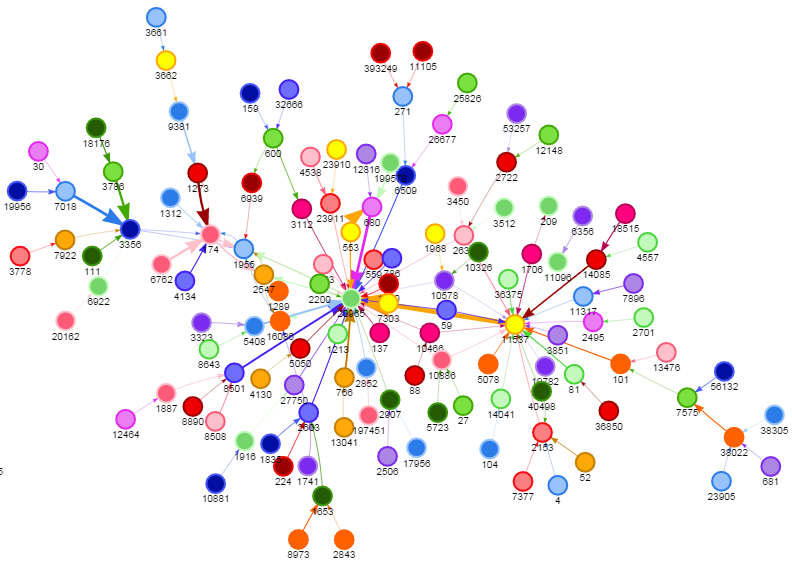
\includegraphics[width=1\textwidth,keepaspectratio]{figures/as-graph.png}

\end{document}
